\documentclass[11pt]{article}
\usepackage{amsmath, amssymb, amscd, amsthm, amsfonts}
\usepackage{graphicx}
\usepackage{hyperref}
\usepackage{commath}
\usepackage{subfig}
\usepackage{float}
\usepackage{natbib}
\usepackage{booktabs}
\oddsidemargin 0pt
\evensidemargin 0pt
\marginparwidth 40pt
\marginparsep 10pt
\topmargin -20pt
\headsep 10pt
\textheight 8.7in
\textwidth 6.65in
\linespread{1.5}

\title{Economics Influence on Housing price Index within Southeast Asian Countries}
\author{Steven Qin\\20819760\\s45qin@uwaterloo.ca \and Tiankai Jiang\\20834939\\t57jiang@uwaterloo.ca}

\date{\today}

\newtheorem{theorem}{Theorem}
\newtheorem{lemma}[theorem]{Lemma}
\newtheorem{conjecture}[theorem]{Conjecture}

\newcommand{\rr}{\mathbb{R}}

\newcommand{\al}{\alpha}
\DeclareMathOperator{\conv}{conv}
\DeclareMathOperator{\aff}{aff}

\makeatletter
\setlength{\@fptop}{0pt}
\makeatother

\begin{document}

\maketitle

For content of Deliverable 3, please go directly to Section \ref{normality_check}

\section{Introduction \& objective}\label{section-introduction}
For the purpose of this project, the objective is to consider various macroeconomic factors, such as the interest rate, GDP growth rate, Consumer Confidence Index (CPI), with an effect on the country wide housing price index. We would subjectively select four individual Southeast Asian countries suitable to represent the overall four national economics level categories ranked by the World Bank. Giving the covid-19 contingency around the world, we would also like to make certain adjustment to the model used to seek a hint on the overall cross-sectional impact.

Target Countries: Japan, People’s Republic of China, Philippine, and Nepal (In descending order of the economics level).

\section{Proposed Model}\label{section-proposedmodel}
$y = \beta_0 + \beta_1x_1 + \beta_2x_2 + ... + \beta_nx_n + \epsilon$

Initially, we choose total population, population density, urban population percentage, unemployment rate, real estate activities, taxes on property, per capita GDP, household final consumption, interest rate\citep{10.2307/23606731, 10.2139/ssrn.2431627, aei297454} as independent variables($x_i$). Dependent variable($y$) is the house price index.

\section{Modeling data}\label{section-proposedmodel}
In this section, we plan to briefly walk through the data modeling and analysis steps which will contribute towards the final delieverable. Using the data from USA as an example, we collected the data of the annual housing price index, GPD per capital, Unemployement rate, and number of building permits.

\begin{figure}[H]
\captionsetup[subfigure]{labelformat=empty}
\centering
\subfloat[]{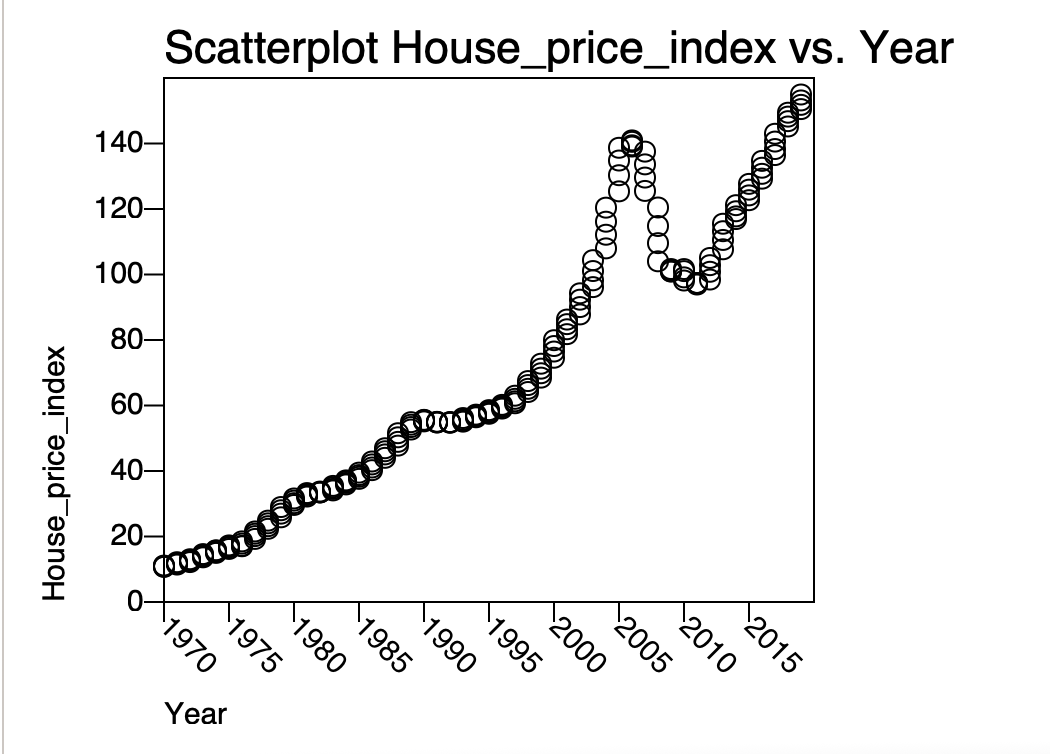
\includegraphics[width=0.24\textwidth]{./image/price_index.png}}
\subfloat[] {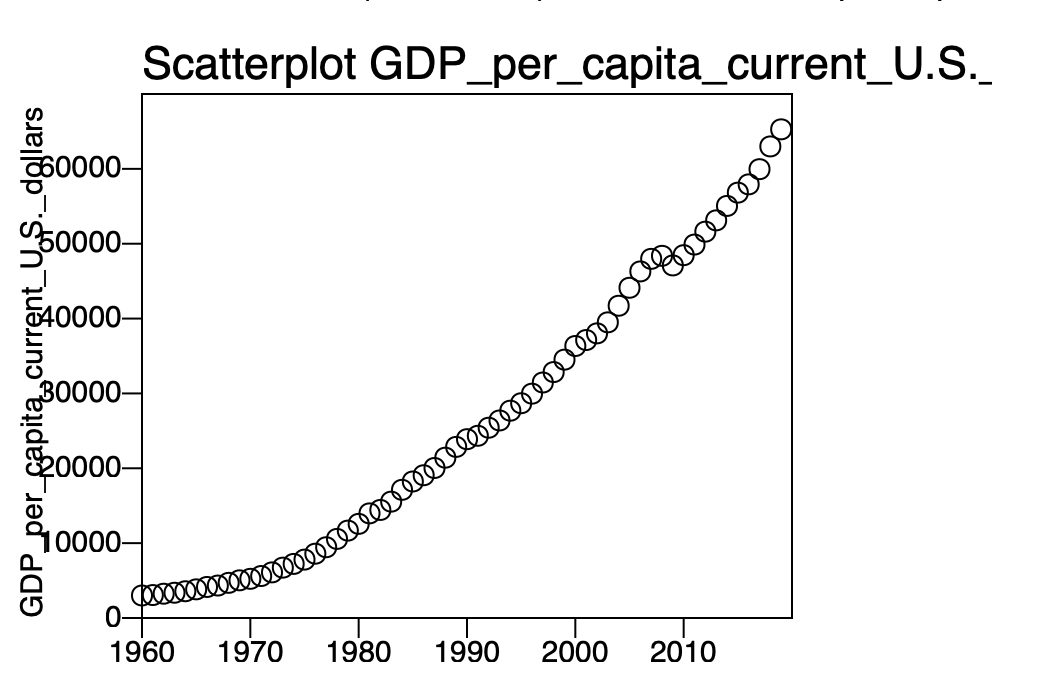
\includegraphics[width=0.24\textwidth]{./image/Gdp.png}}
\subfloat[] {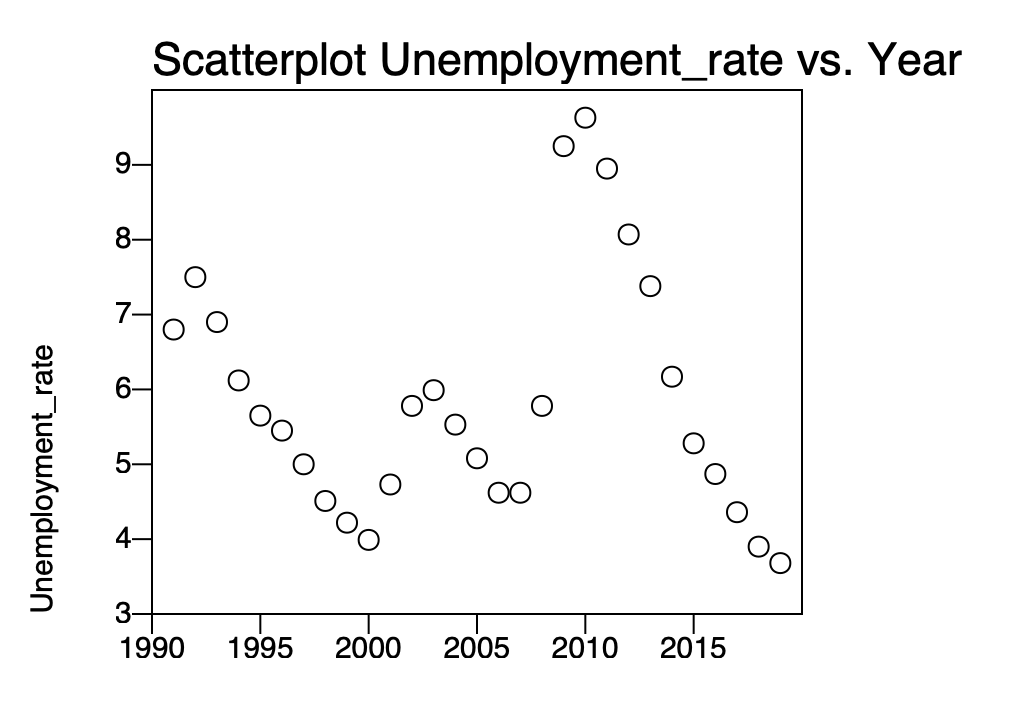
\includegraphics[width=0.24\textwidth]{./image/Unemployment.png}}
\subfloat[] {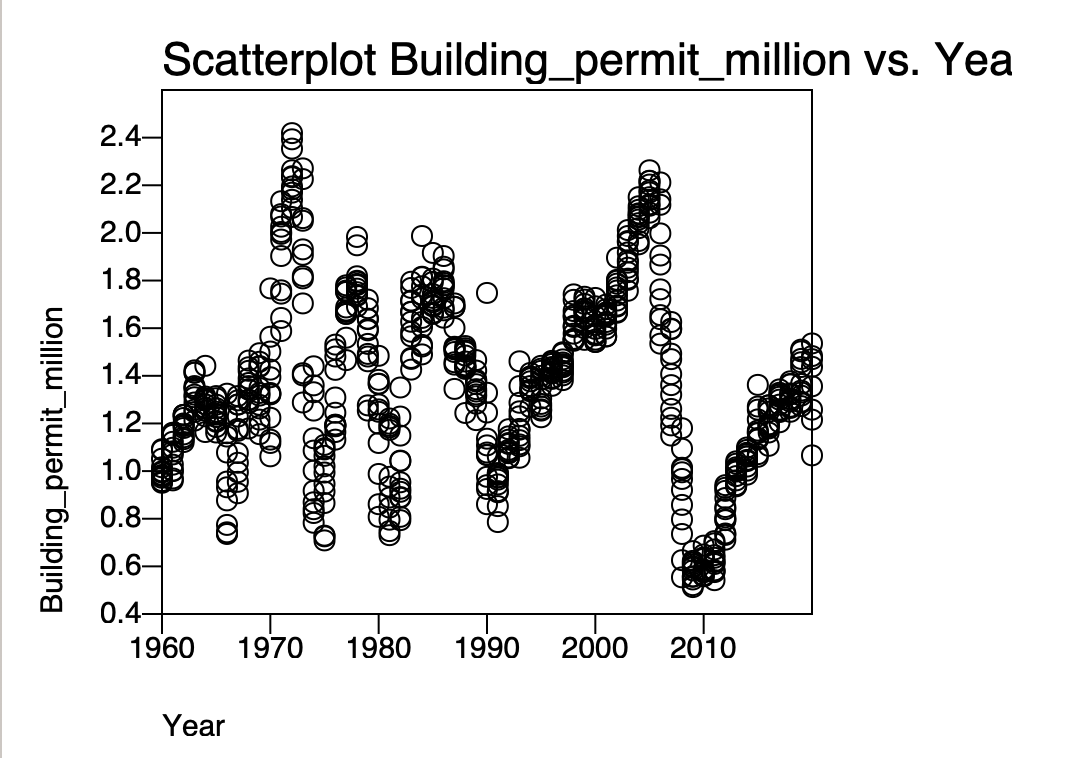
\includegraphics[width=0.24\textwidth]{./image/building_permit.png}}
\end{figure}

As shown above, the housing price has an overall uptrend, with a periodic recession during the 2008 financial crisis. A similar pattern appeals to the growth of GDP per capita. On the other hand, the national unemployment rate and the number of issued building permits are cyclical under the influence of the national economic, world economic environment, and other factors. Although displayed differently, we can still capture similarity characteristics. For instance, unemployment is recorded at a historical high during the financial crisis(The unemployment rate is a lagging indicator of the business cycle. Therefore, we see the historical high is recorded in 2010, but the upward trend obviously started at approximately coincide with the crisis). In the same way, a pattern can also seem for building permits. 
Hence, we will choose these three mentioned factors as the independent variables for the HPI in the model and analysis of the data based upon it.  

\section{Data Tables and variable discription}\label{section-datatable}

\begin{table}[H]
\begin{tabular}{|c|c|}
\hline
\textbf{Variable Name}                                                                              & \textbf{Description} \\ \hline
\begin{tabular}[c]{@{}c@{}}GDP per capita, \\ current U.S. dollars\end{tabular}                     & Ratio                \\ \hline
\begin{tabular}[c]{@{}c@{}}Household consumption \\ as percent of GDP\end{tabular}                  & Ratio                \\ \hline
Unemployment rate                                                                                   & Ratio                \\ \hline
Personal income tax rate                                                                            & Ratio                \\ \hline
\begin{tabular}[c]{@{}c@{}}Taxes on goods \\ and services, percent \\ of total revenue\end{tabular} & Ratio                \\ \hline
\begin{tabular}[c]{@{}c@{}}Real interest rate: \\ Bank lending rate \\ minus inflation\end{tabular} & Ratio                \\ \hline
\begin{tabular}[c]{@{}c@{}}Population size, \\ in millions\end{tabular}                             & Ordinal              \\ \hline
\begin{tabular}[c]{@{}c@{}}Percent urban \\ population\end{tabular}                                 & Ratio                \\ \hline
\begin{tabular}[c]{@{}c@{}}Population density, \\ people per square km\end{tabular}                 & Ratio                \\ \hline
Annual HPI                                                                                          & Ratio                \\ \hline
\end{tabular}
\end{table}

\begin{flushleft}
\begin{tabular}{lrrrr}
\toprule
{} & \multicolumn{4}{l}{GDP per capita, current U.S. dollars} \\
{} &                                 mean &       min &       max &          std \\
Country     &                                      &           &           &              \\
\midrule
China       &                          7307.242727 &   3832.24 &  10261.68 &  2081.428551 \\
India       &                          1619.529091 &   1101.96 &   2104.15 &   308.639618 \\
Japan       &                         41070.663636 &  34524.47 &  48603.48 &  4334.089586 \\
Philippines &                          2821.324545 &   1905.89 &   3485.08 &   468.083442 \\
\bottomrule
\end{tabular}

\vspace{2em}

\begin{tabular}{lrrrr}
\toprule
{} & \multicolumn{4}{l}{Household consumption as percent of GDP} \\
{} &                                    mean &    min &    max &       std \\
Country     &                                         &        &        &           \\
\midrule
China       &                               36.779091 &  34.33 &  38.67 &  1.680770 \\
India       &                               57.820000 &  54.72 &  60.24 &  1.754685 \\
Japan       &                               57.220000 &  55.44 &  58.96 &  1.431642 \\
Philippines &                               72.208182 &  70.19 &  73.21 &  0.859032 \\
\bottomrule
\end{tabular}

\vspace{2em}

\begin{tabular}{lrrrr}
\toprule
{} & \multicolumn{4}{l}{Unemployment rate} \\
{} &              mean &   min &   max &       std \\
Country     &                   &       &       &           \\
\midrule
China       &          4.524545 &  4.28 &  4.72 &  0.131329 \\
India       &          5.542727 &  5.33 &  5.67 &  0.121416 \\
Japan       &          3.691818 &  2.29 &  5.10 &  0.999488 \\
Philippines &          3.134545 &  2.15 &  3.86 &  0.597518 \\
\bottomrule
\end{tabular}

\vspace{2em}

\begin{tabular}{lrrrr}
\toprule
{} & \multicolumn{4}{l}{Personal income tax rate} \\
{} &                     mean &   min &   max &       std \\
Country     &                          &       &       &           \\
\midrule
China       &                45.000000 &  45.0 &  45.0 &  0.000000 \\
India       &                33.363636 &  30.0 &  36.0 &  2.766685 \\
Japan       &                52.454545 &  50.0 &  56.0 &  2.841255 \\
Philippines &                32.545455 &  32.0 &  35.0 &  1.213560 \\
\bottomrule
\end{tabular}

\vspace{2em}

\begin{tabular}{lrrrr}
\toprule
{} & \multicolumn{4}{l}{Taxes on goods and services, percent of total revenue} \\
{} &                                                  mean &    min &    max &        std \\
Country     &                                                       &        &        &            \\
\midrule
China       &                                          46.751818 &  32.88 &  63.37 &  13.755032 \\
India       &                                          27.733636 &  21.68 &  31.76 &   3.586517 \\
Japan       &                                          36.270000 &  32.73 &  38.52 &   1.661614 \\
Philippines &                                          25.441818 &  22.67 &  27.28 &   1.401990 \\
\bottomrule
\end{tabular}

\vspace{2em}

\begin{tabular}{lrrrr}
\toprule
{} & \multicolumn{4}{l}{Real interest rate: Bank lending rate minus inflation} \\
{} &                                                  mean &   min &   max &       std \\
Country     &                                                       &       &       &           \\
\midrule
China       &                                           2.354545 & -1.40 &  5.53 &  2.353985 \\
India       &                                           4.380000 & -1.98 &  7.56 &  2.846601 \\
Japan       &                                           1.348182 & -0.98 &  3.56 &  1.429467 \\
Philippines &                                           3.963636 &  2.29 &  6.34 &  1.504980 \\
\bottomrule
\end{tabular}

\vspace{2em}

\begin{tabular}{lrrrr}
\toprule
{} & \multicolumn{4}{l}{Population size, in millions} \\
{} &                         mean &      min &      max &        std \\
Country     &                              &          &          &            \\
\midrule
China       &                  1364.741818 &  1331.26 &  1397.71 &  22.591435 \\
India       &                  1294.262727 &  1217.73 &  1366.42 &  49.124745 \\
Japan       &                   127.274545 &   126.26 &   128.07 &   0.601438 \\
Philippines &                   100.386364 &    92.41 &   108.12 &   5.253632 \\
\bottomrule
\end{tabular}

\vspace{2em}

\begin{tabular}{lrrrr}
\toprule
{} & \multicolumn{4}{l}{Percent urban population} \\
{} &                     mean &    min &    max &       std \\
Country     &                          &        &        &           \\
\midrule
China       &                54.210000 &  47.88 &  60.31 &  4.120017 \\
India       &                32.442727 &  30.59 &  34.47 &  1.286826 \\
Japan       &                91.204545 &  89.99 &  91.70 &  0.478359 \\
Philippines &                46.128182 &  45.33 &  47.15 &  0.625297 \\
\bottomrule
\end{tabular}

\vspace{2em}

\begin{tabular}{lrrrr}
\toprule
{} & \multicolumn{4}{l}{Population density, people per square km} \\
{} &                                     mean &  min &  max &        std \\
Country     &                                          &      &      &            \\
\midrule
China       &                               145.272727 &  142 &  148 &   2.327699 \\
India       &                               434.636364 &  410 &  455 &  15.279219 \\
Japan       &                               349.272727 &  347 &  351 &   1.420627 \\
Philippines &                               336.000000 &  310 &  358 &  16.540859 \\
\bottomrule
\end{tabular}

\vspace{2em}

\begin{tabular}{lrrrr}
\toprule
{} & \multicolumn{4}{l}{Annual HPI} \\
{} &        mean &    min &     max &        std \\
Country     &             &        &         &            \\
\midrule
China       &  113.938182 &  94.76 &  139.24 &  14.024913 \\
India       &  200.740909 &  89.42 &  291.59 &  71.904262 \\
Japan       &  104.033636 &  98.27 &  112.84 &   5.198198 \\
Philippines &  160.984545 &  98.40 &  296.50 &  61.288144 \\
\bottomrule
\end{tabular}
\end{flushleft}

\section{Certainty of Variable}\label{section-Certainty}
HPI is a commonly used indicator by investors to keep a palus on the broader economic trend. In the data source we found, HPI is displayed quarterly. Therefore we chose the number in December to represent the current year's change in price by the rule of the laspeyres index. The rise and fall is interrelated with the economic. In general, price rise may be interpreted as a form of accumulating wealth from the day-to-day operation. Hence such events often leads to lower unemployment rate and high Consumer Confidence Index (CCI) that leads to high consumptions. Furthermore, it paves the way for a boost in the domestic aggregate demand and GDP\citep{aei297454}. In purpose of this project, my team would select independent variables that have direct implications on the domestic household disposable income level. Factors choosen are listed and described below. 
\begin{itemize}
\item Demand variables: GDP in the form of \(GDP = C + I + G - (X-M)\) where is C is household consumption, I is private domestic investment, G is net government expenditure, X-M represents the net of export. 
\item Price variables: CPI and GDP deflator where as \(deflator = (Nominal GDP / Real GPD) * 100 \)
\item Interest rates (Real): \(real interest rate = nominal interest rate - inflation rate\) where the inflation rate captures the percentage change in the CPI and nominal interest rate shows the domestica policy rate set by each domestic monetary agency. 
\item Mortgage loan and unemployment rate as representation of CCI
\item For taxes, a few illustrative items that are related to household disposable income were chosen from the data base. Such as personal income tax rate, tax on goods and services.
\item For each country, we also included total population size, percent urban population, and population density. These elements were chosen because a higher population, usually leads to high density which would increase housing prices. Besides, the urban population also provides a significant contribution to house prices for it's a common scene that metropolitan has a higher housing price than the countryside.
\item Data Source: 
    \begin{itemize}
        \item \href{https://kidb.adb.org/kidb/onlineQuery}{KIDB: Key indicators regarding people, economy, transport, energy, environment, government}
        \item \href{https://www.theglobaleconomy.com/}{Global Economy}
    \end{itemize}

\end{itemize}     

\section{Check Normality of the Dependent Variable}\label{normality_check}
We use Kolmolgorov-Smirnoff test to check normality of the dependent variable.
$$D=\underset{1 \leq i \leq N}{\max}(F(Y_i)-\frac{i-1}{N},\frac{i}{N}-F(Y_i))$$
$H_0$: The variable is normally distributed.\\
$H_a$: The variable is not normally distributed.\\
In the table below, 
$$Cumulative=Rank$$ 
$$Expected=\frac{Cumulative}{Count}$$ 
$$(Rank-1)/n=\frac{Cumulative-1}{Count}$$
$$Actual=NORM.DIST(x, {\bar X}, stddev, true)$$
$$Difference=\abs{Actual-(Rank-1)/n}$$
Maximum=MAX(Difference), which is the result of the Kolmolgorov-Smirnoff test. For China, India, Japan, Philippines, the result are \textbf{0.1873, 0.1224, 0.1338, 0.1536} respectively. According to the One-Sample Kolmogorov-Smirnov Table, when $n=11$ and $\alpha=0.05$, the critical value $D_{n,a}=0.3912$. All four results are less than the critical value. Therefore, we failed to reject the $H_0$. The dependent variable is normally distributed.
\begin{figure}[H]
\begin{center}
    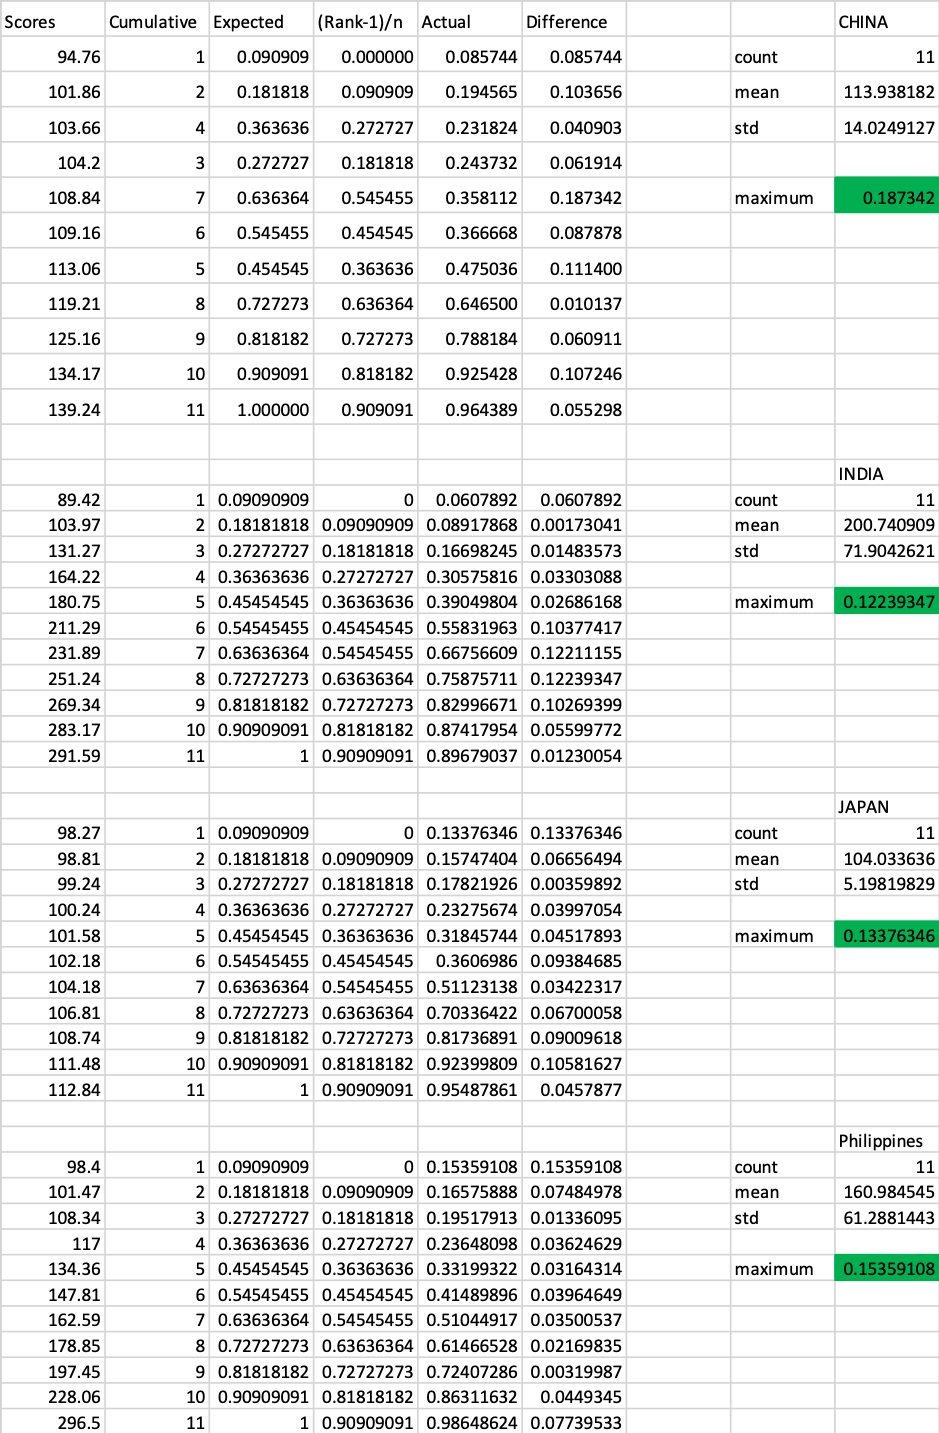
\includegraphics[width=0.85\textwidth]{./image/KSTest.png}
\end{center}
\end{figure}

\section{Mean Comparison of the Dependent Variable}\label{mean_comparison}
Perform one-tail two sample independent t-test on all four countries. Therefore, there are 6 comparisons in total.\\
Let $\mu_1$ denotes the average HPI of the country in the first column, $\mu_2$ denotes the average HPI of the country in the second column.\\
$H_0: \mu_1\geq \mu_2$\\
$H_a: \mu_1< \mu_2$\\
$df=11+11-2=20$, the critical value for an one-tail t-test when $\alpha=0.05$ is $t_{crit}=1.725$.\\
The results are as follows:
\begin{figure}[H]
\begin{center}
    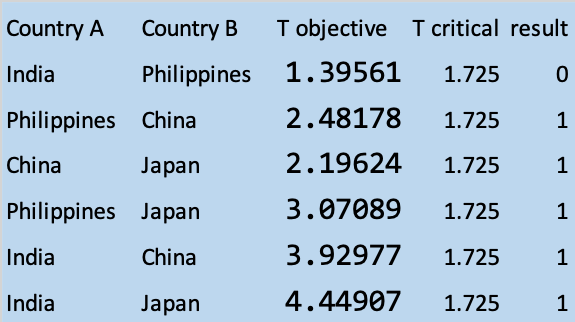
\includegraphics[width=0.85\textwidth]{./image/TTest.png}
\end{center}
\end{figure}

For the comparison between India and Philippines, $t_{obj}=1.3956<t_{crit}$. We failed to reject $H_0$ and conclude that there is not enough evidence to show that the average HPI of Philippines is greater than that of India. For all other five comparisions, $t_{obj}>t_{crit}$, we reject $H_0$ and conclude that the HPI of the country in the second column is indeed greater than that in the first column.

\section{Regression Analysis}\label{regression_analysis}
We have mentioned in the previous section that there are lots of independent variables that may influence the house price index. It is obvious that we cannot use all of them for regression. Therefore, the first step is to select the proper independent variables. We have the following constraints:
\begin{enumerate}
    \item It is not possible to fit all four countries in a same linear function with the same coefficients, however, we should at least use the same independent variables for four regressions. Otherwise, the results are just four separate models without comparability.
    \item When selecting the independent variables for regression, any selected variable should be strongly correlated with HPI.
    \item When selecting the independent variables for regression, all selected variables should not be strongly correlated with each other.
\end{enumerate}
Our strategy is\citep{Feature}:
\begin{enumerate}
    \item We construct the Pearson Correlation Table of all variables for all four countries. And remove a variable if in any tables, the correlation between that variable and the annual HPI is less or equal to 0.5.
    \item After the first step, all variables left are strongly correlated with annual HPI. We construct the Pearson Correlation Table again, this time, for all independent variables left. And we only pick one from a group, if that group of variables are strongly correlated with each other (here we pick r=0.7). 
\end{enumerate}
We use China as an example, below is the Pearson Correlation Table constructed in step 1. Here actually we only use the annual HPI row (indicate by a green arrow):
\begin{figure}[H]
\begin{center}
    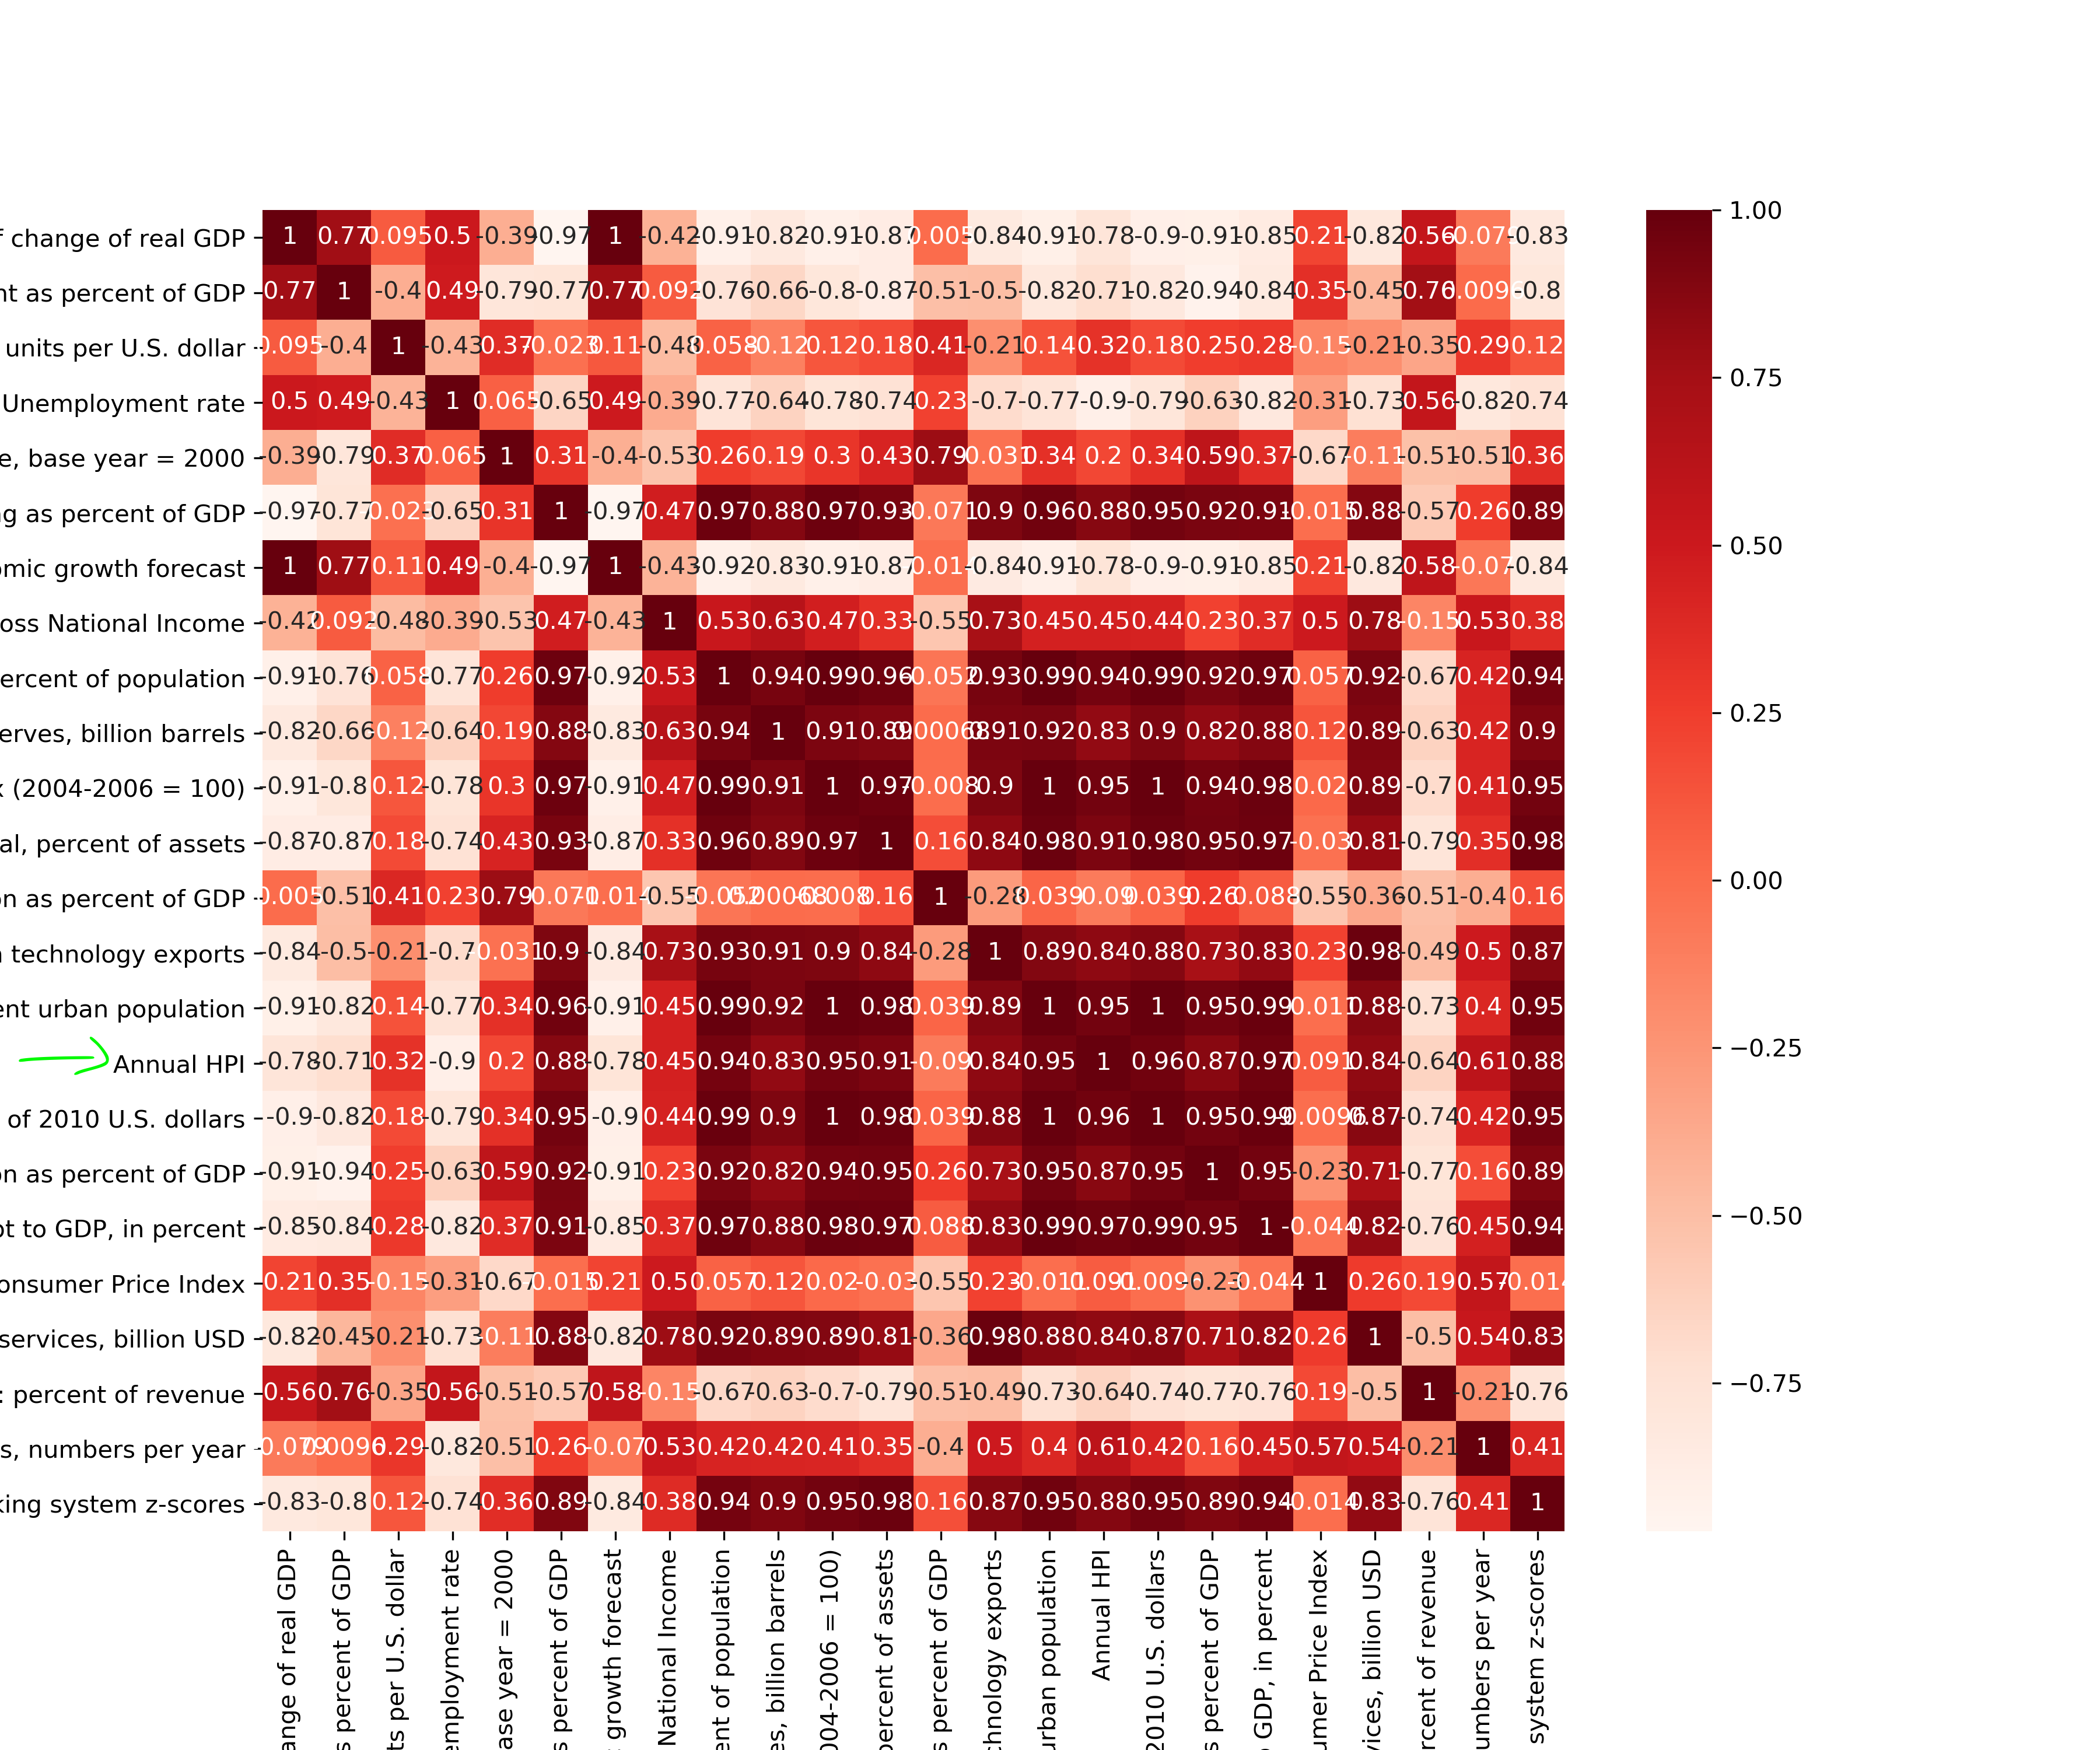
\includegraphics[width=1.0\textwidth]{./image/CorrelationTable1.png}
\end{center}
\end{figure}
After doing this step for all four countries, we plot the correlation table for all variables left:
\begin{figure}[H]
\begin{center}
    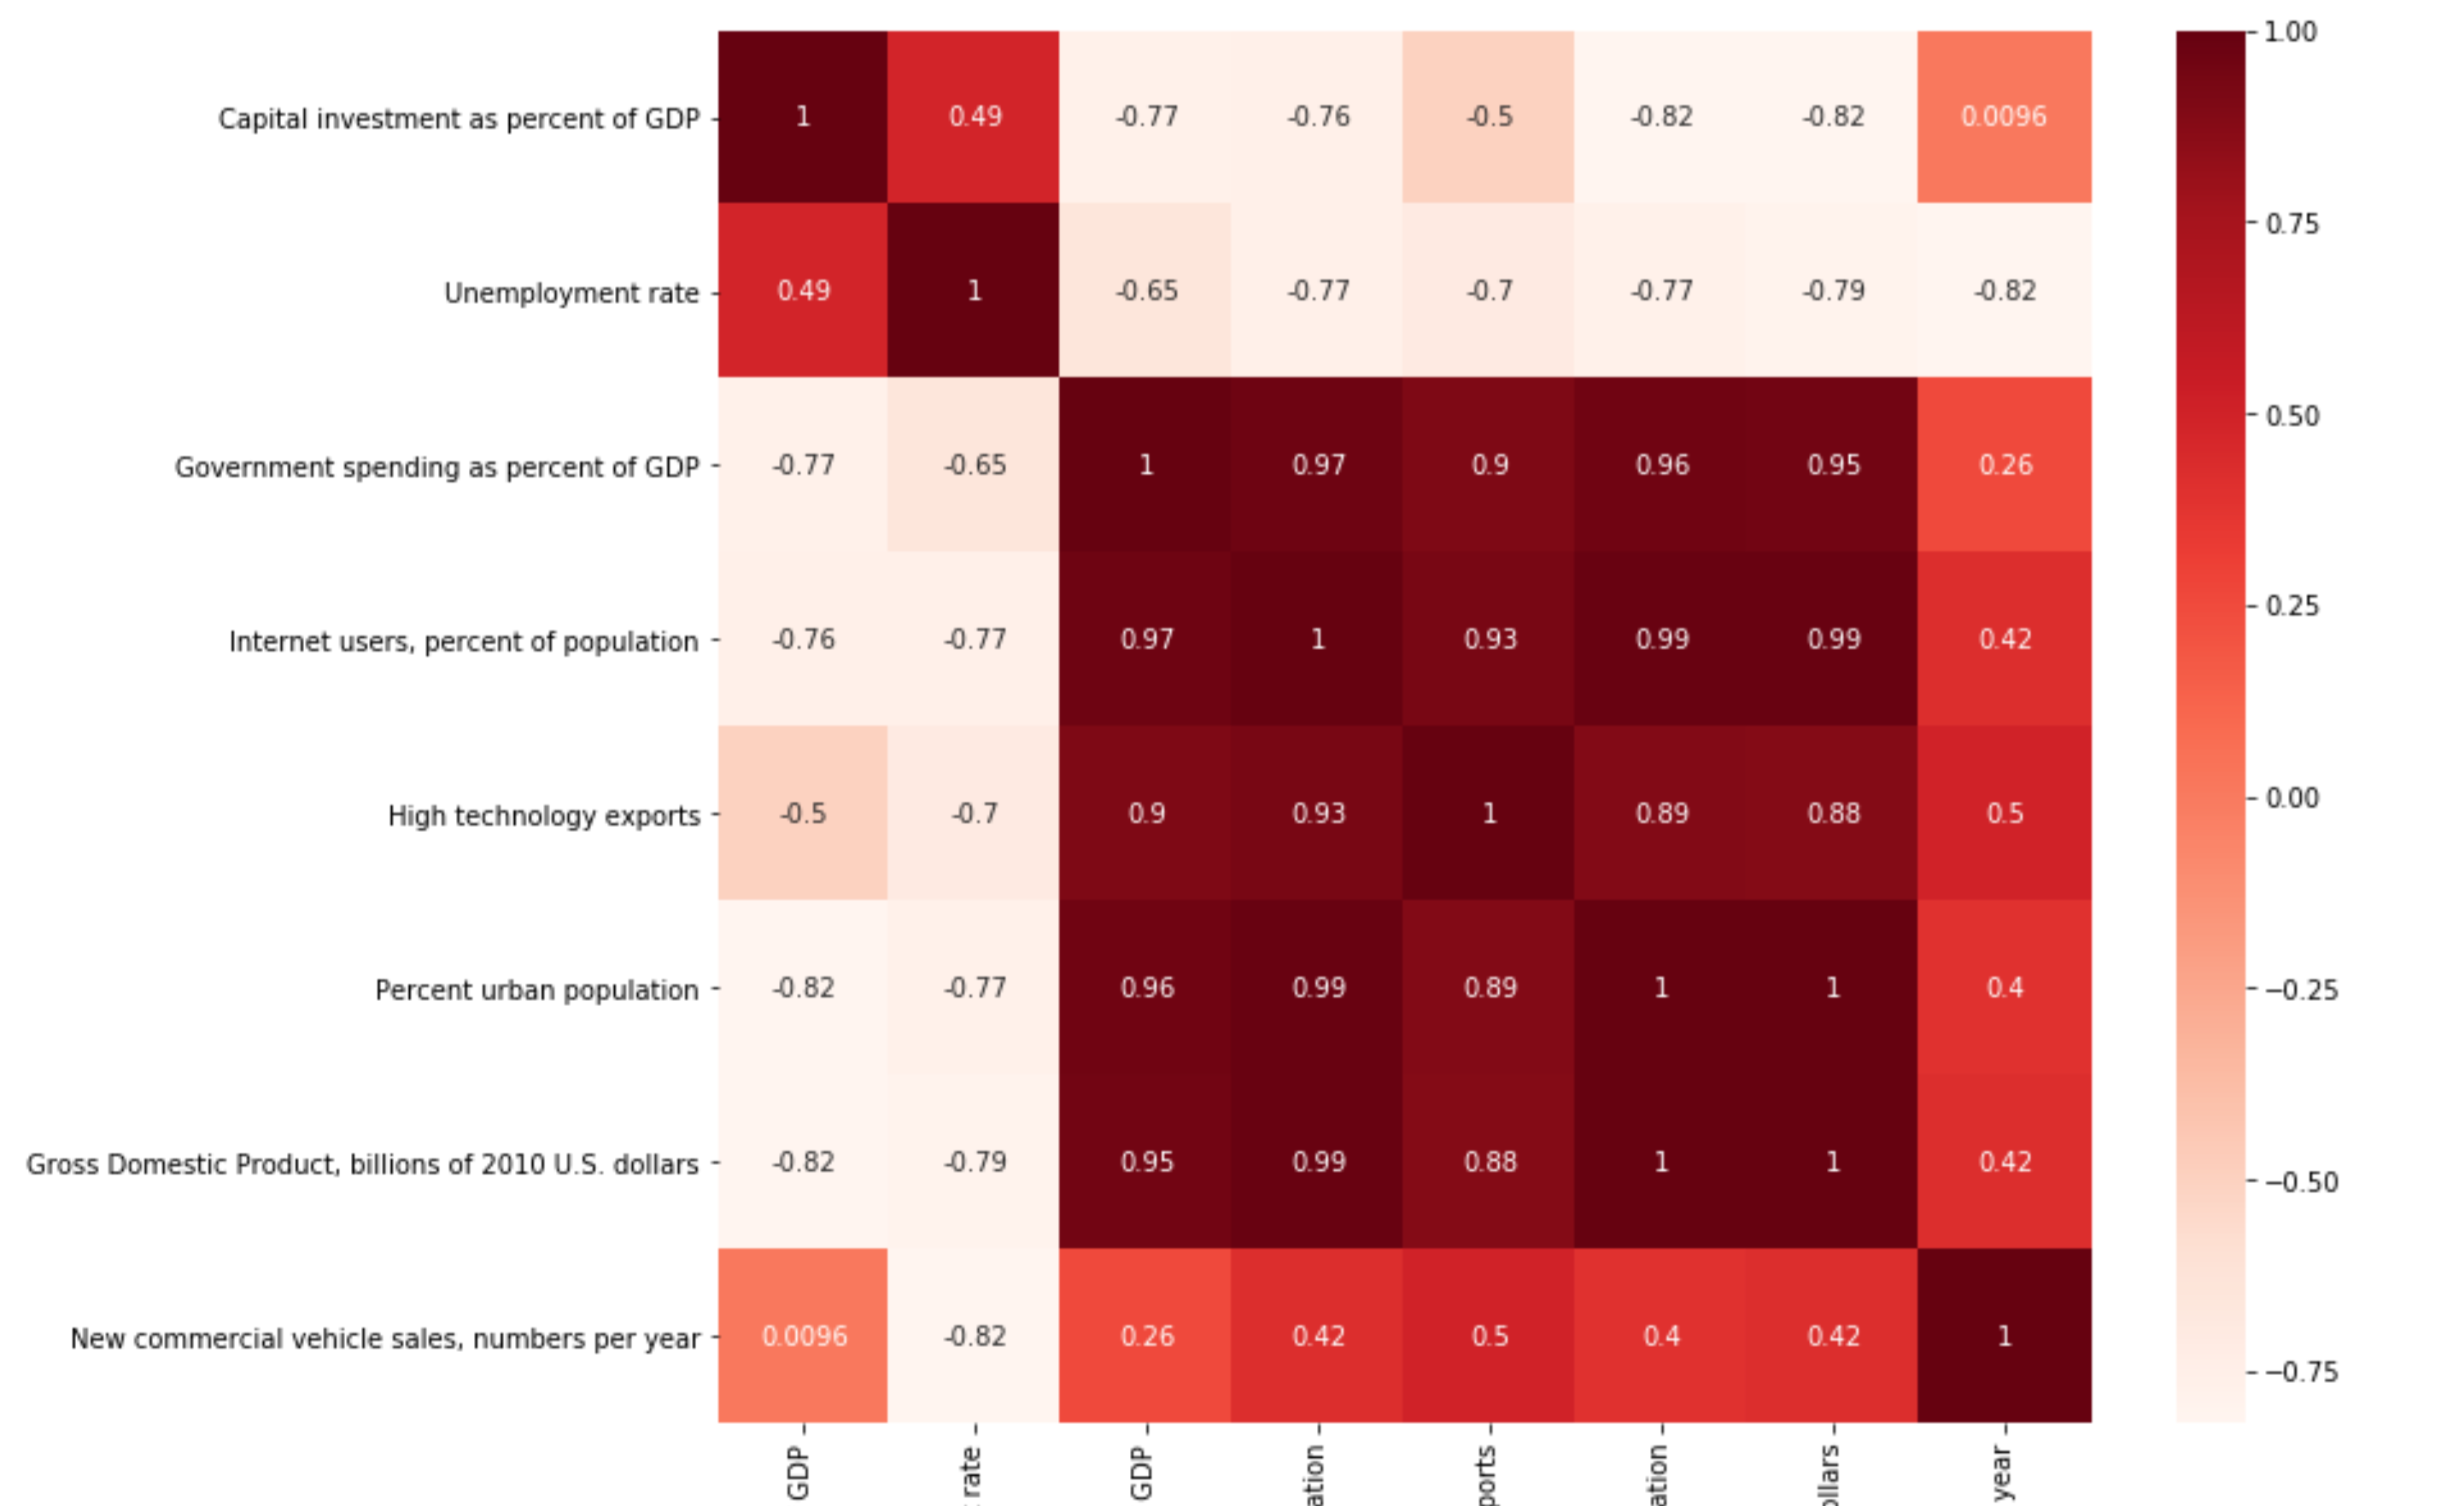
\includegraphics[width=1.0\textwidth]{./image/CorrelationTable2.png}
\end{center}
\end{figure}
Lots of independent variables are strongly correlated, which does not satisfy the assumption of linear regression. Here we pick only Unemployment rate and Government spending as percent of GDP (row 2 and row 3).

Using the OLS funtion in python package statsmodels, we perform linear regression for four countries respectively, below is the result:

Japan:
\begin{figure}[H]
\begin{center}
    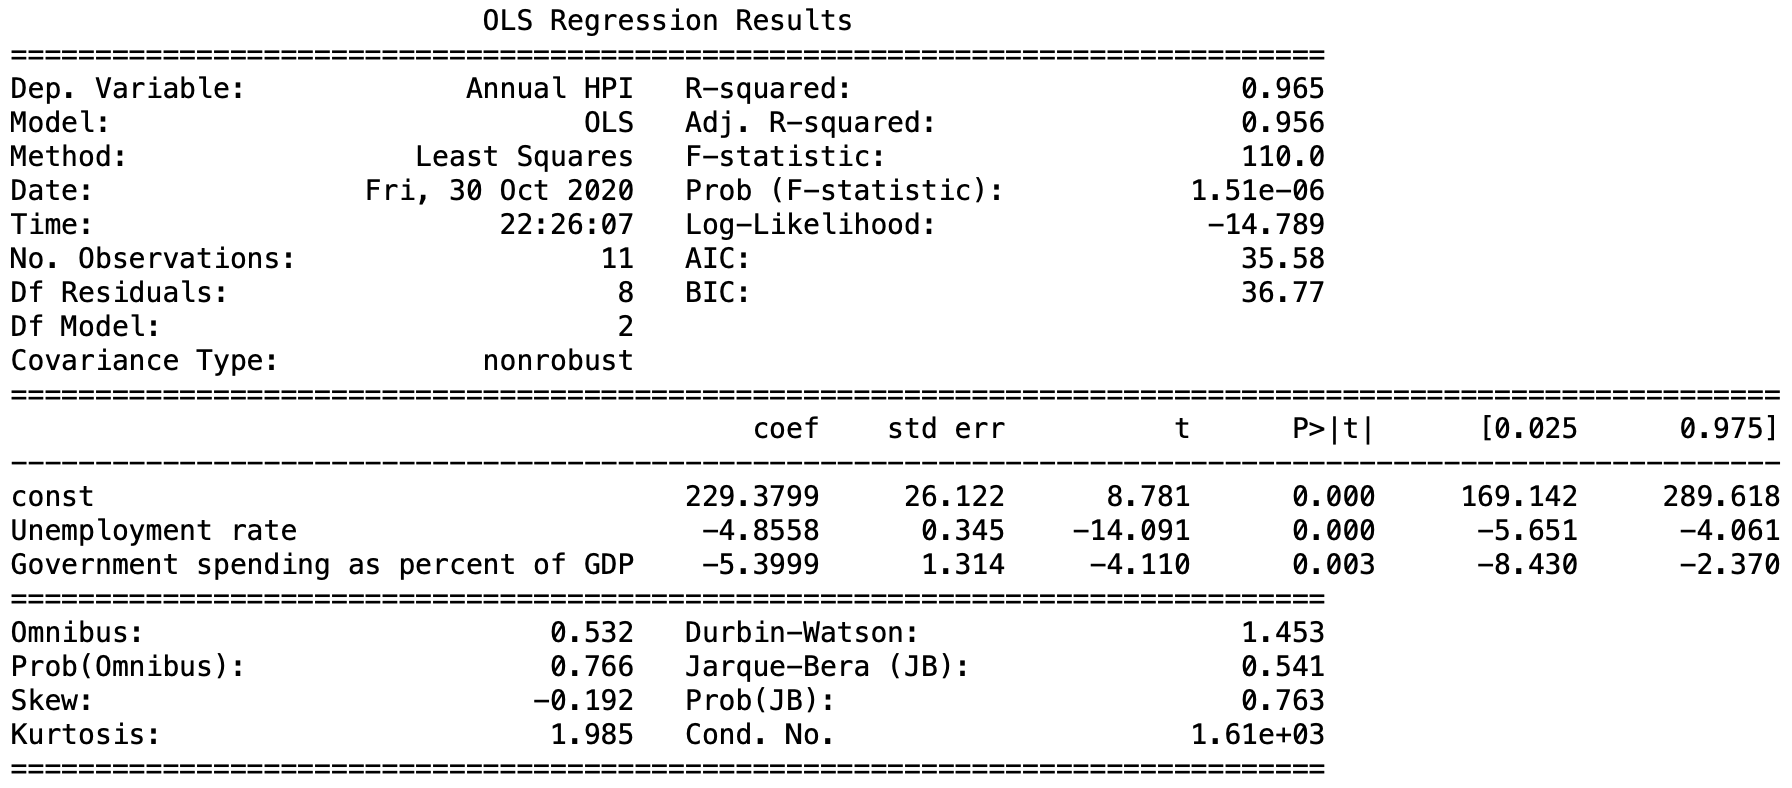
\includegraphics[width=0.8\textwidth]{./image/Reg_JPN.png}
\end{center}
\end{figure}

China:
\begin{figure}[H]
\begin{center}
    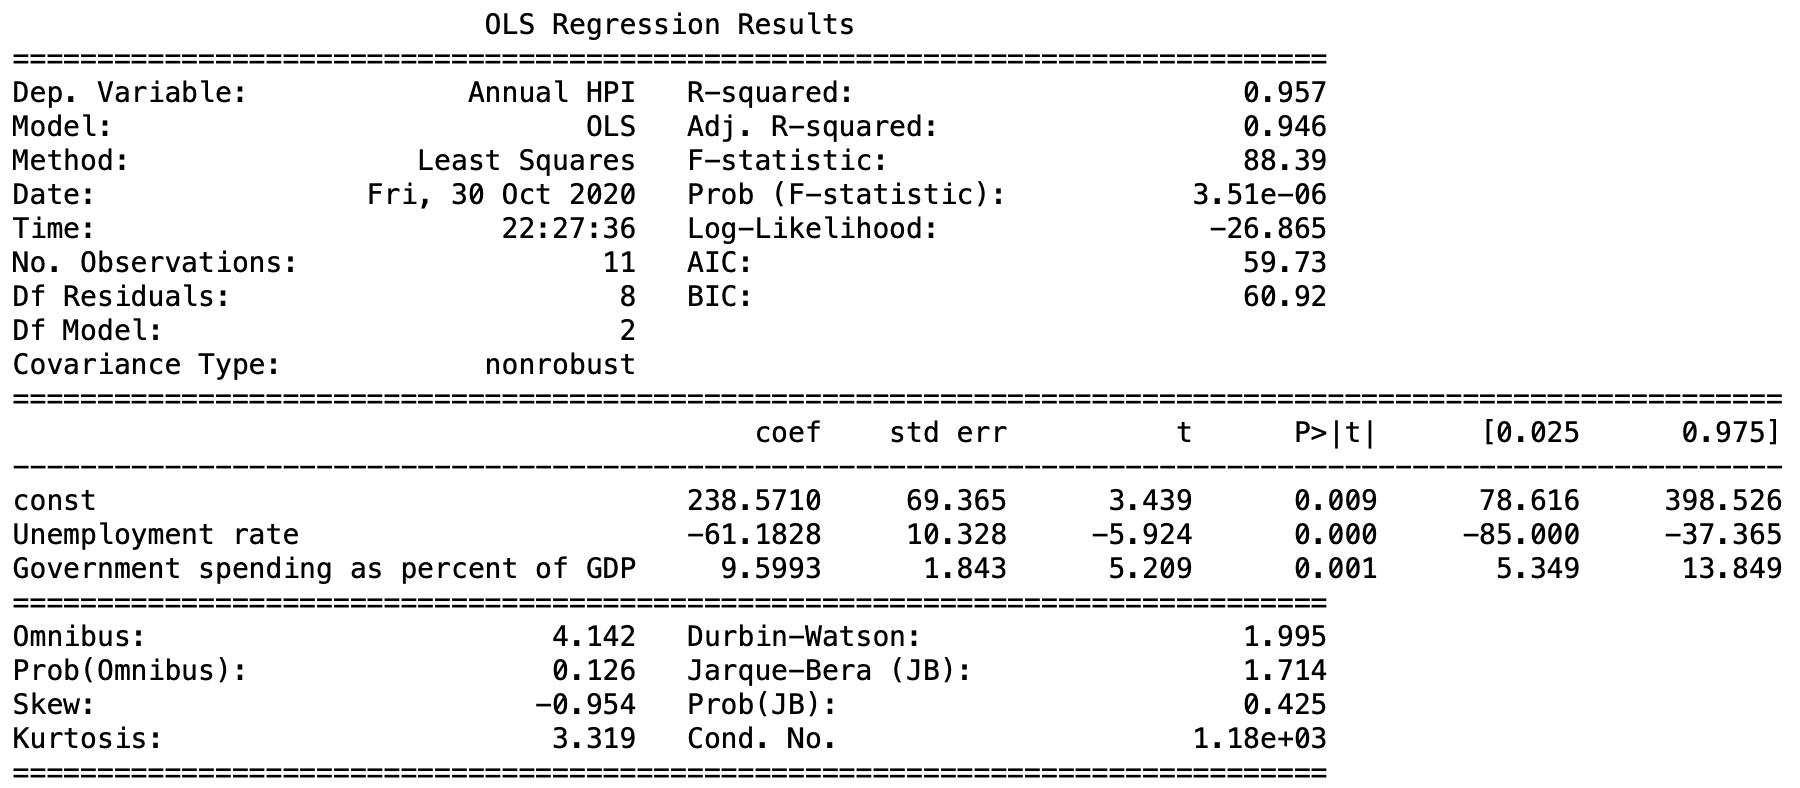
\includegraphics[width=0.8\textwidth]{./image/Reg_CHN.png}
\end{center}
\end{figure}

Philippines:
\begin{figure}[H]
\begin{center}
    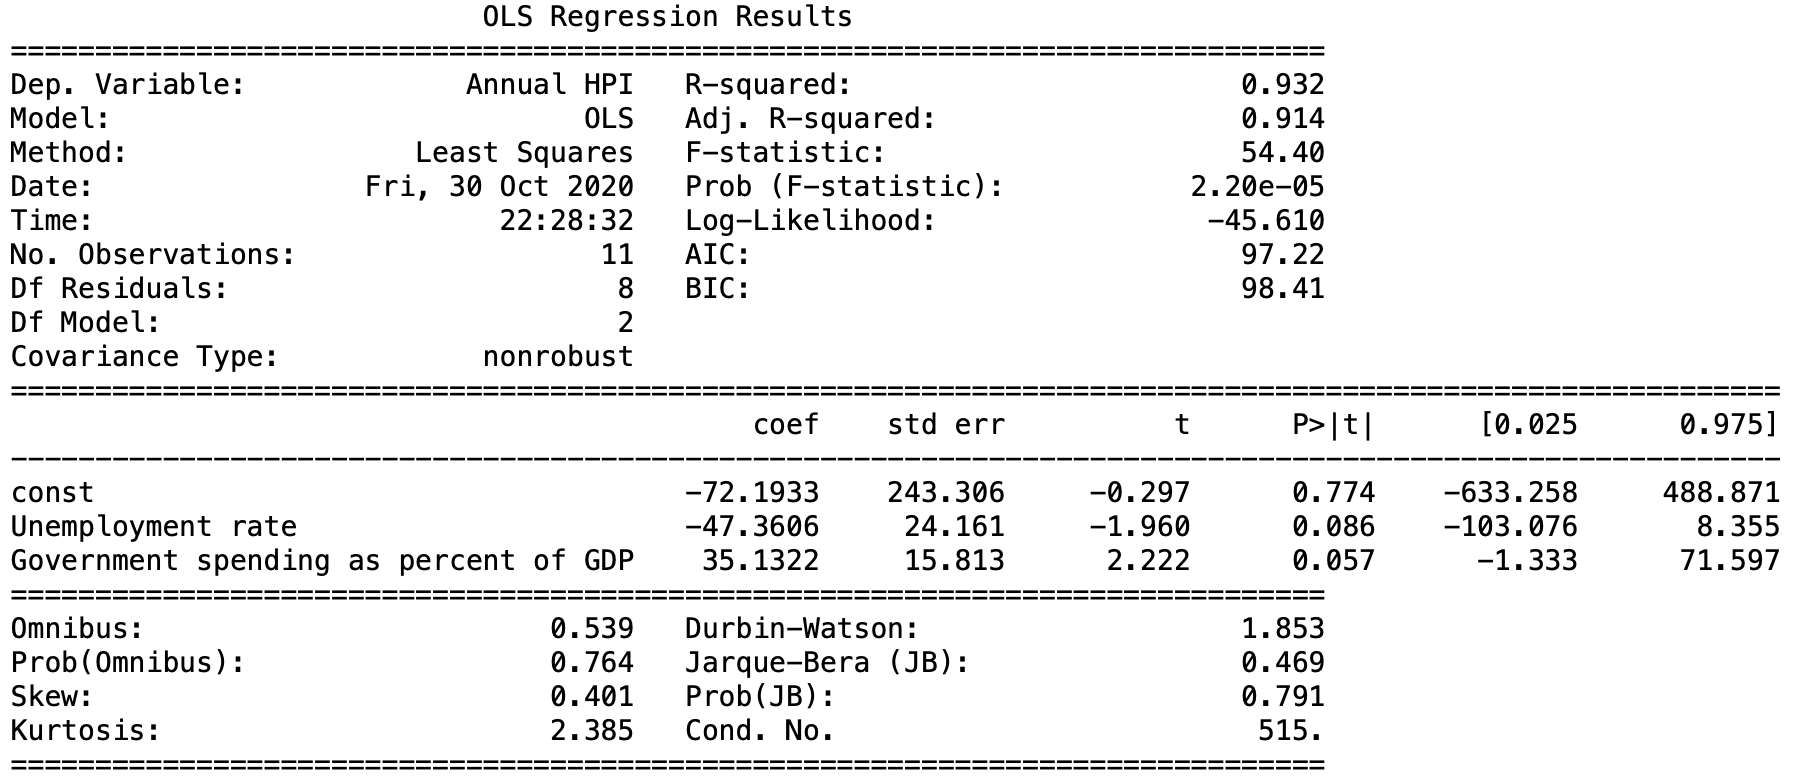
\includegraphics[width=0.8\textwidth]{./image/Reg_PHL.png}
\end{center}
\end{figure}

India:
\begin{figure}[H]
\begin{center}
    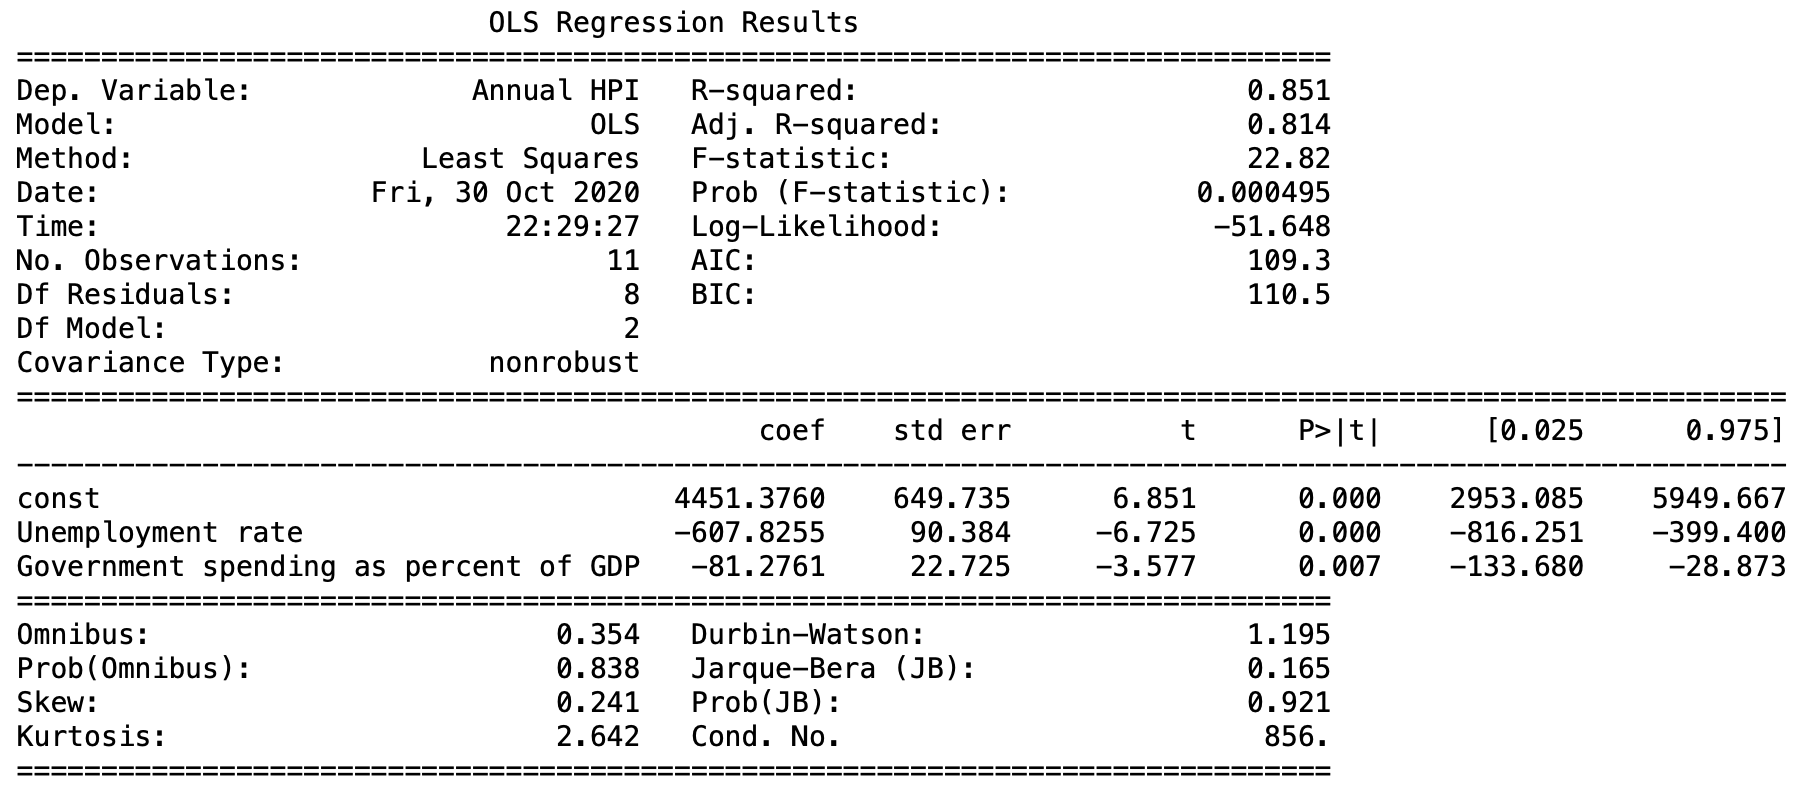
\includegraphics[width=0.8\textwidth]{./image/Reg_IND.png}
\end{center}
\end{figure}

For Philippines, the P-value of the constant is 0.774, which is abnormal. That's because the unemployment rate and government spending are strongly correlated in Philippines. However, as we are finding an universal model for all four countries, we have to make some compromise. For now, this is the temporary solution, maybe we can find a better model later.

\section{Residuals Analysis}\label{residuals_analysis}
We can get the residual of the regression from model.resid if using OLS in statsmodels. Checking the normality of the residual is the same as checking the normality of the dependent variable. We will leave out the manual calculation and use kstest package and shapiro package from scipy.stats directly.

The result of the Kolmolgorov-Smirnoff test is:
\begin{itemize}
    \item Japan: KstestResult(statistic=0.1599800489339369, pvalue=0.9409537714586017)
    \item China: KstestResult(statistic=0.319720396192871, pvalue=0.16866155548919362)
    \item Philippines: KstestResult(statistic=0.5445262080791782, pvalue=0.0013854288164271162)
    \item India: KstestResult(statistic=0.5454545454545454, pvalue=0.0013494428782933796)
\end{itemize}

which means that except for Japan, the residuals of other three countries are not normally distributed.

For the purpose of this project, heteroskedasticity represents the level of volatility in the market. For example, there exists an correlation between the housing price and inflation, money supply. Although we may assume the real price of the HPI remains constant during the observation, the norminal price, which is reflected in HPI, continuous to grow. Hence, we choose to believe the volitity would increase along the HPI\citep{Heteroskedasticity1,Heteroskedasticity2}.

We create the residual plots for all four countries:

Japan:
\begin{figure}[H]
\captionsetup[subfigure]{labelformat=empty}
\centering
\subfloat[]{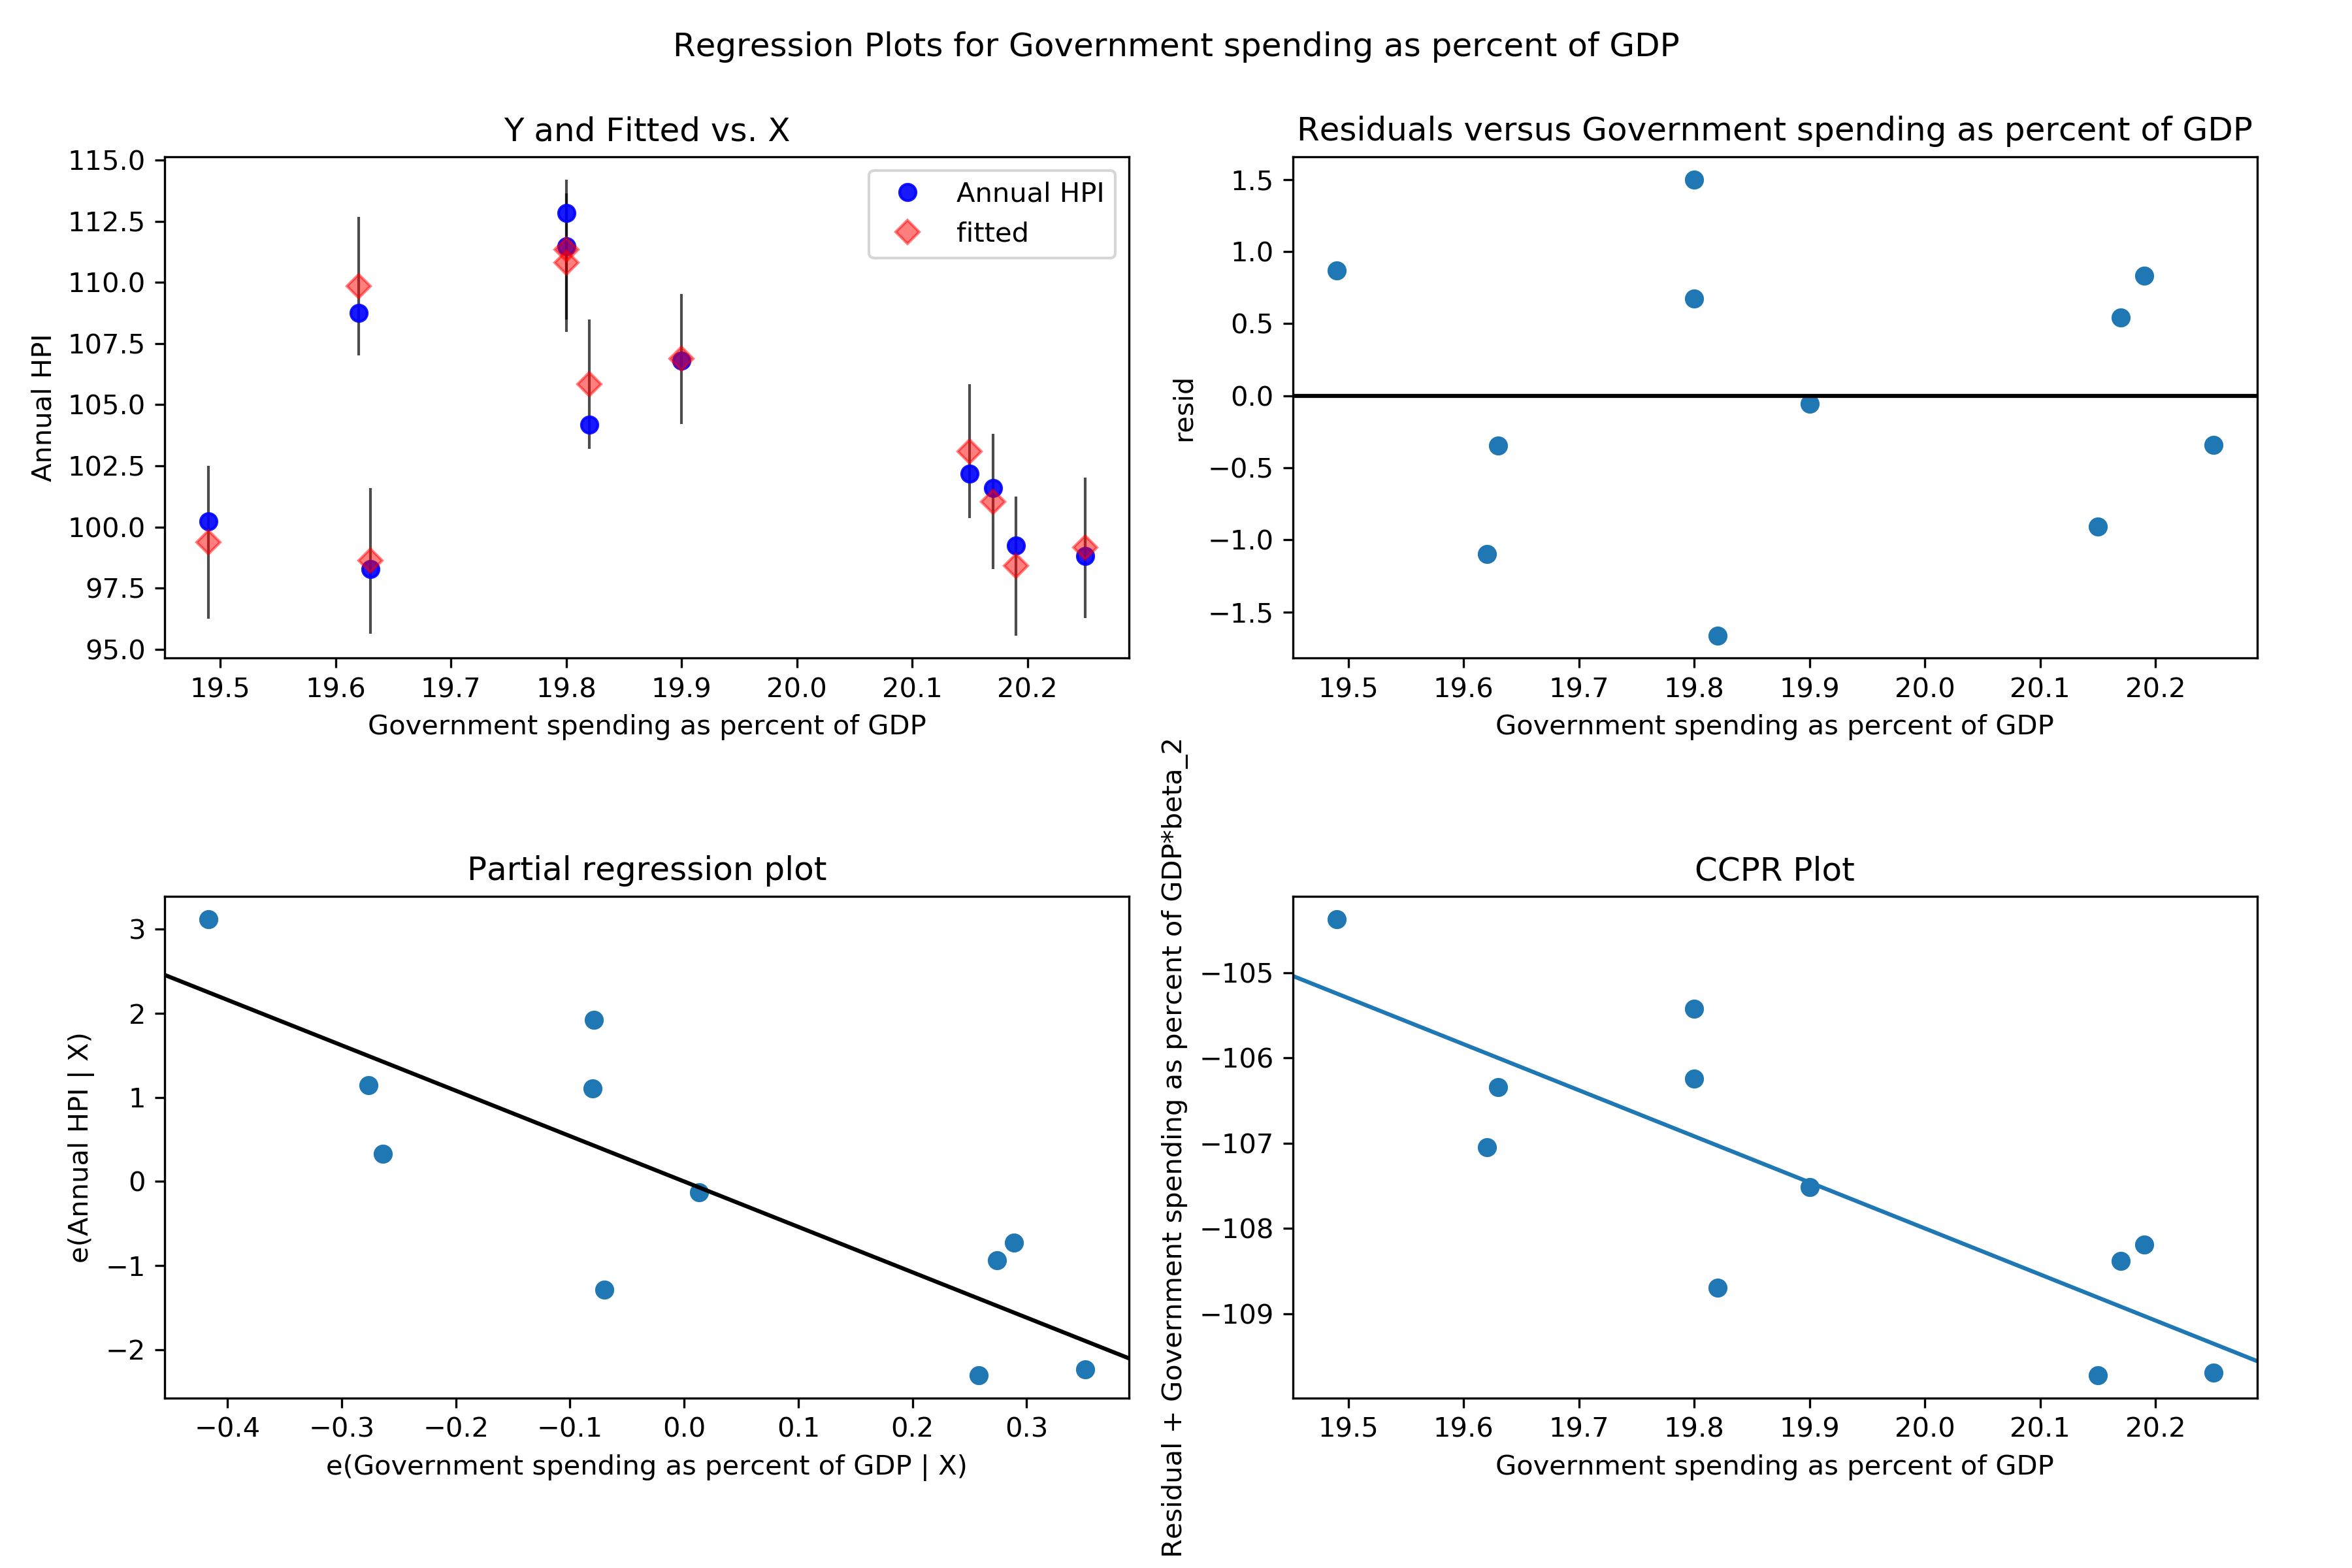
\includegraphics[width=0.49\textwidth]{./image/Resid_gs_JPN.png}}
\subfloat[] {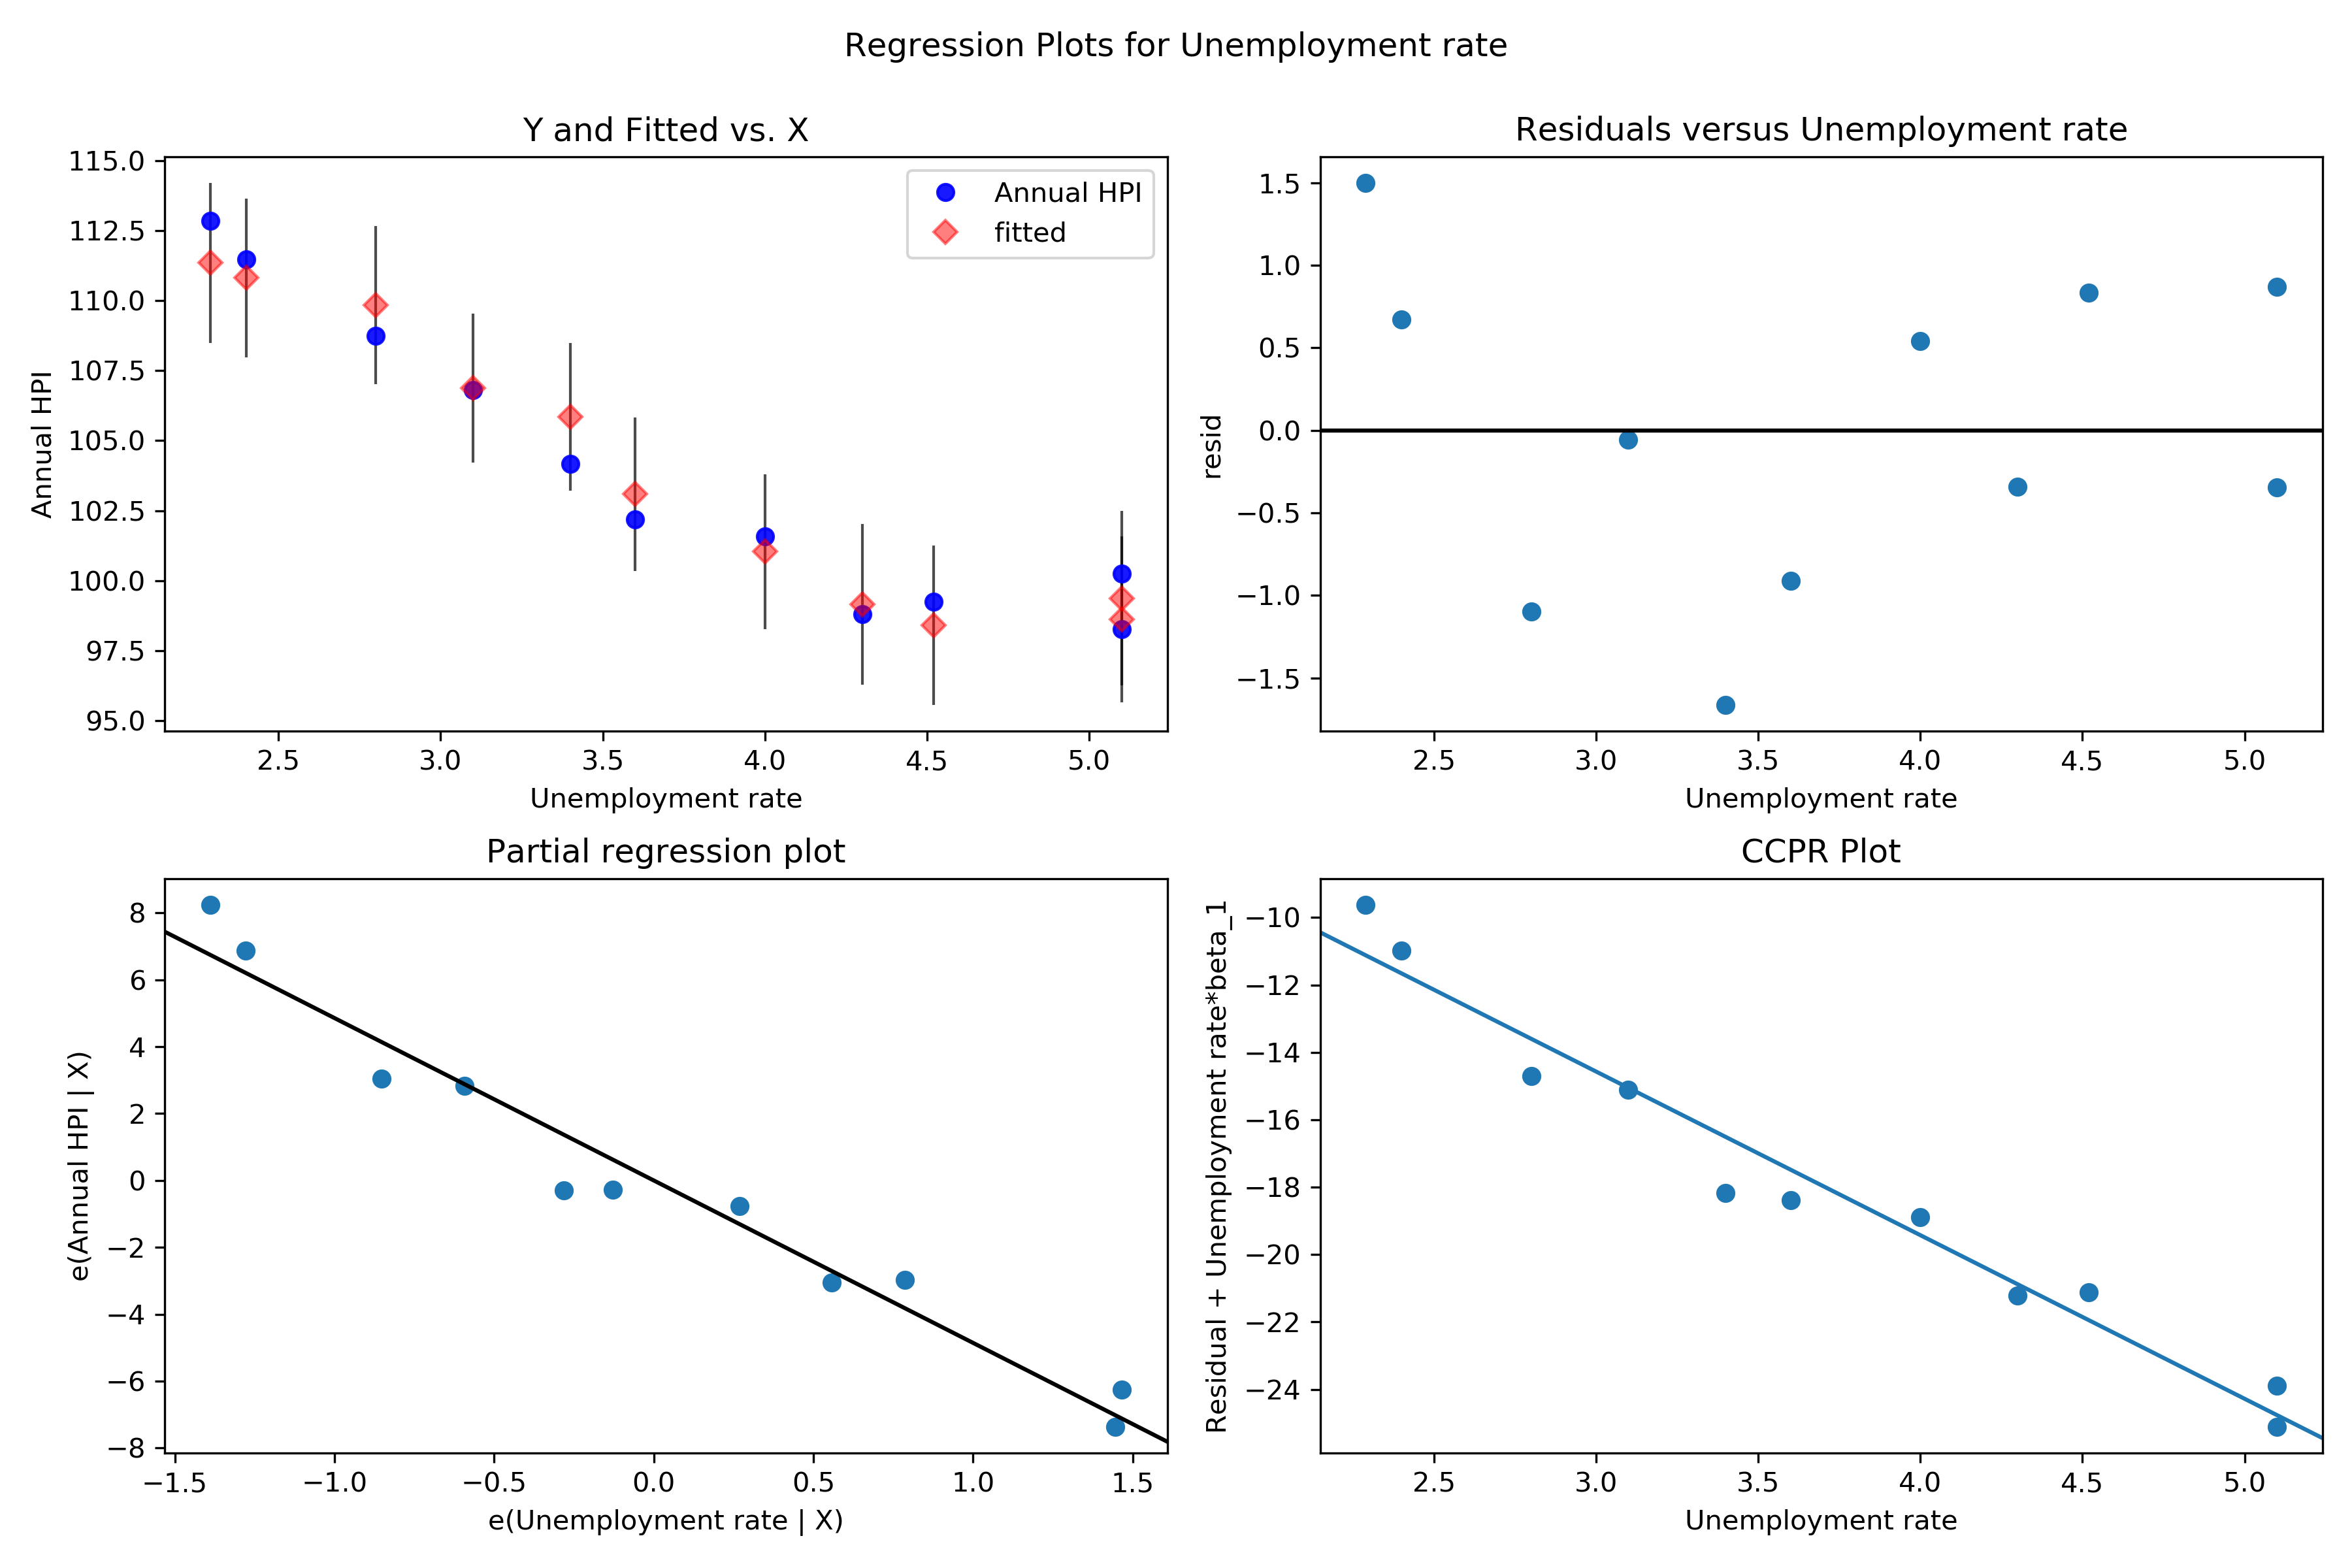
\includegraphics[width=0.49\textwidth]{./image/Resid_unemployment_JPN.png}}
\end{figure}

China:
\begin{figure}[H]
\captionsetup[subfigure]{labelformat=empty}
\centering
\subfloat[]{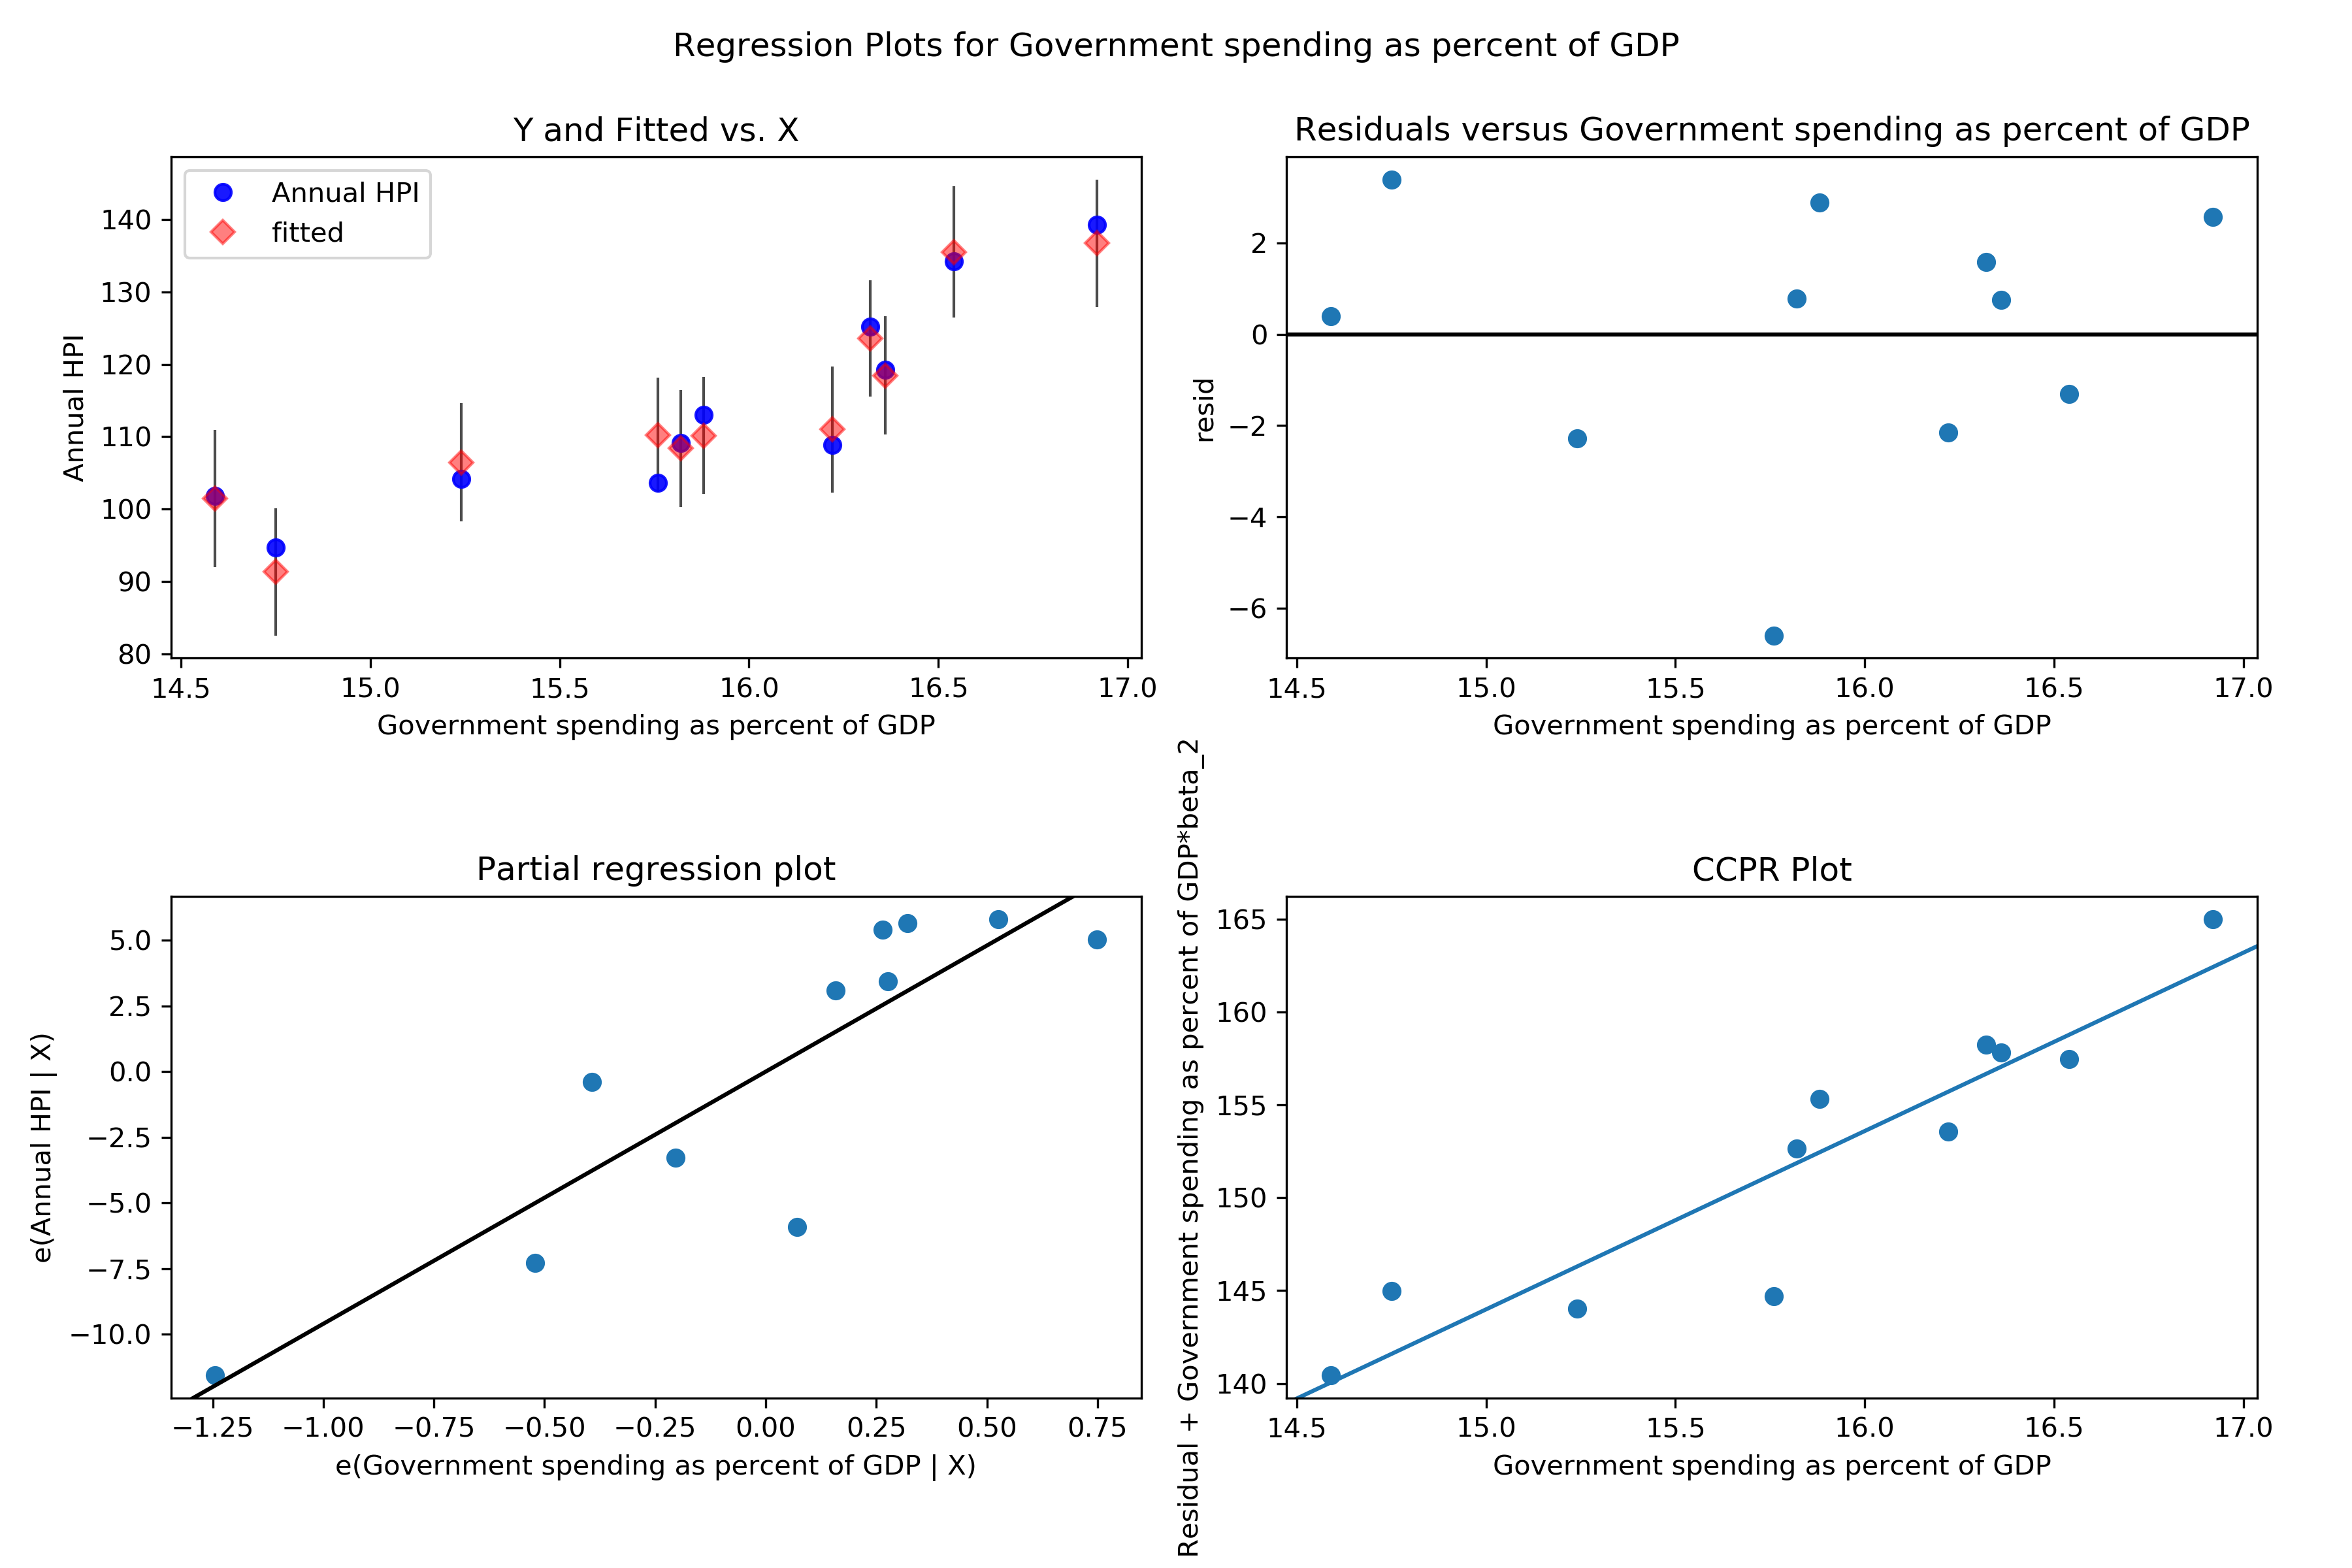
\includegraphics[width=0.49\textwidth]{./image/Resid_gs_CHN.png}}
\subfloat[] {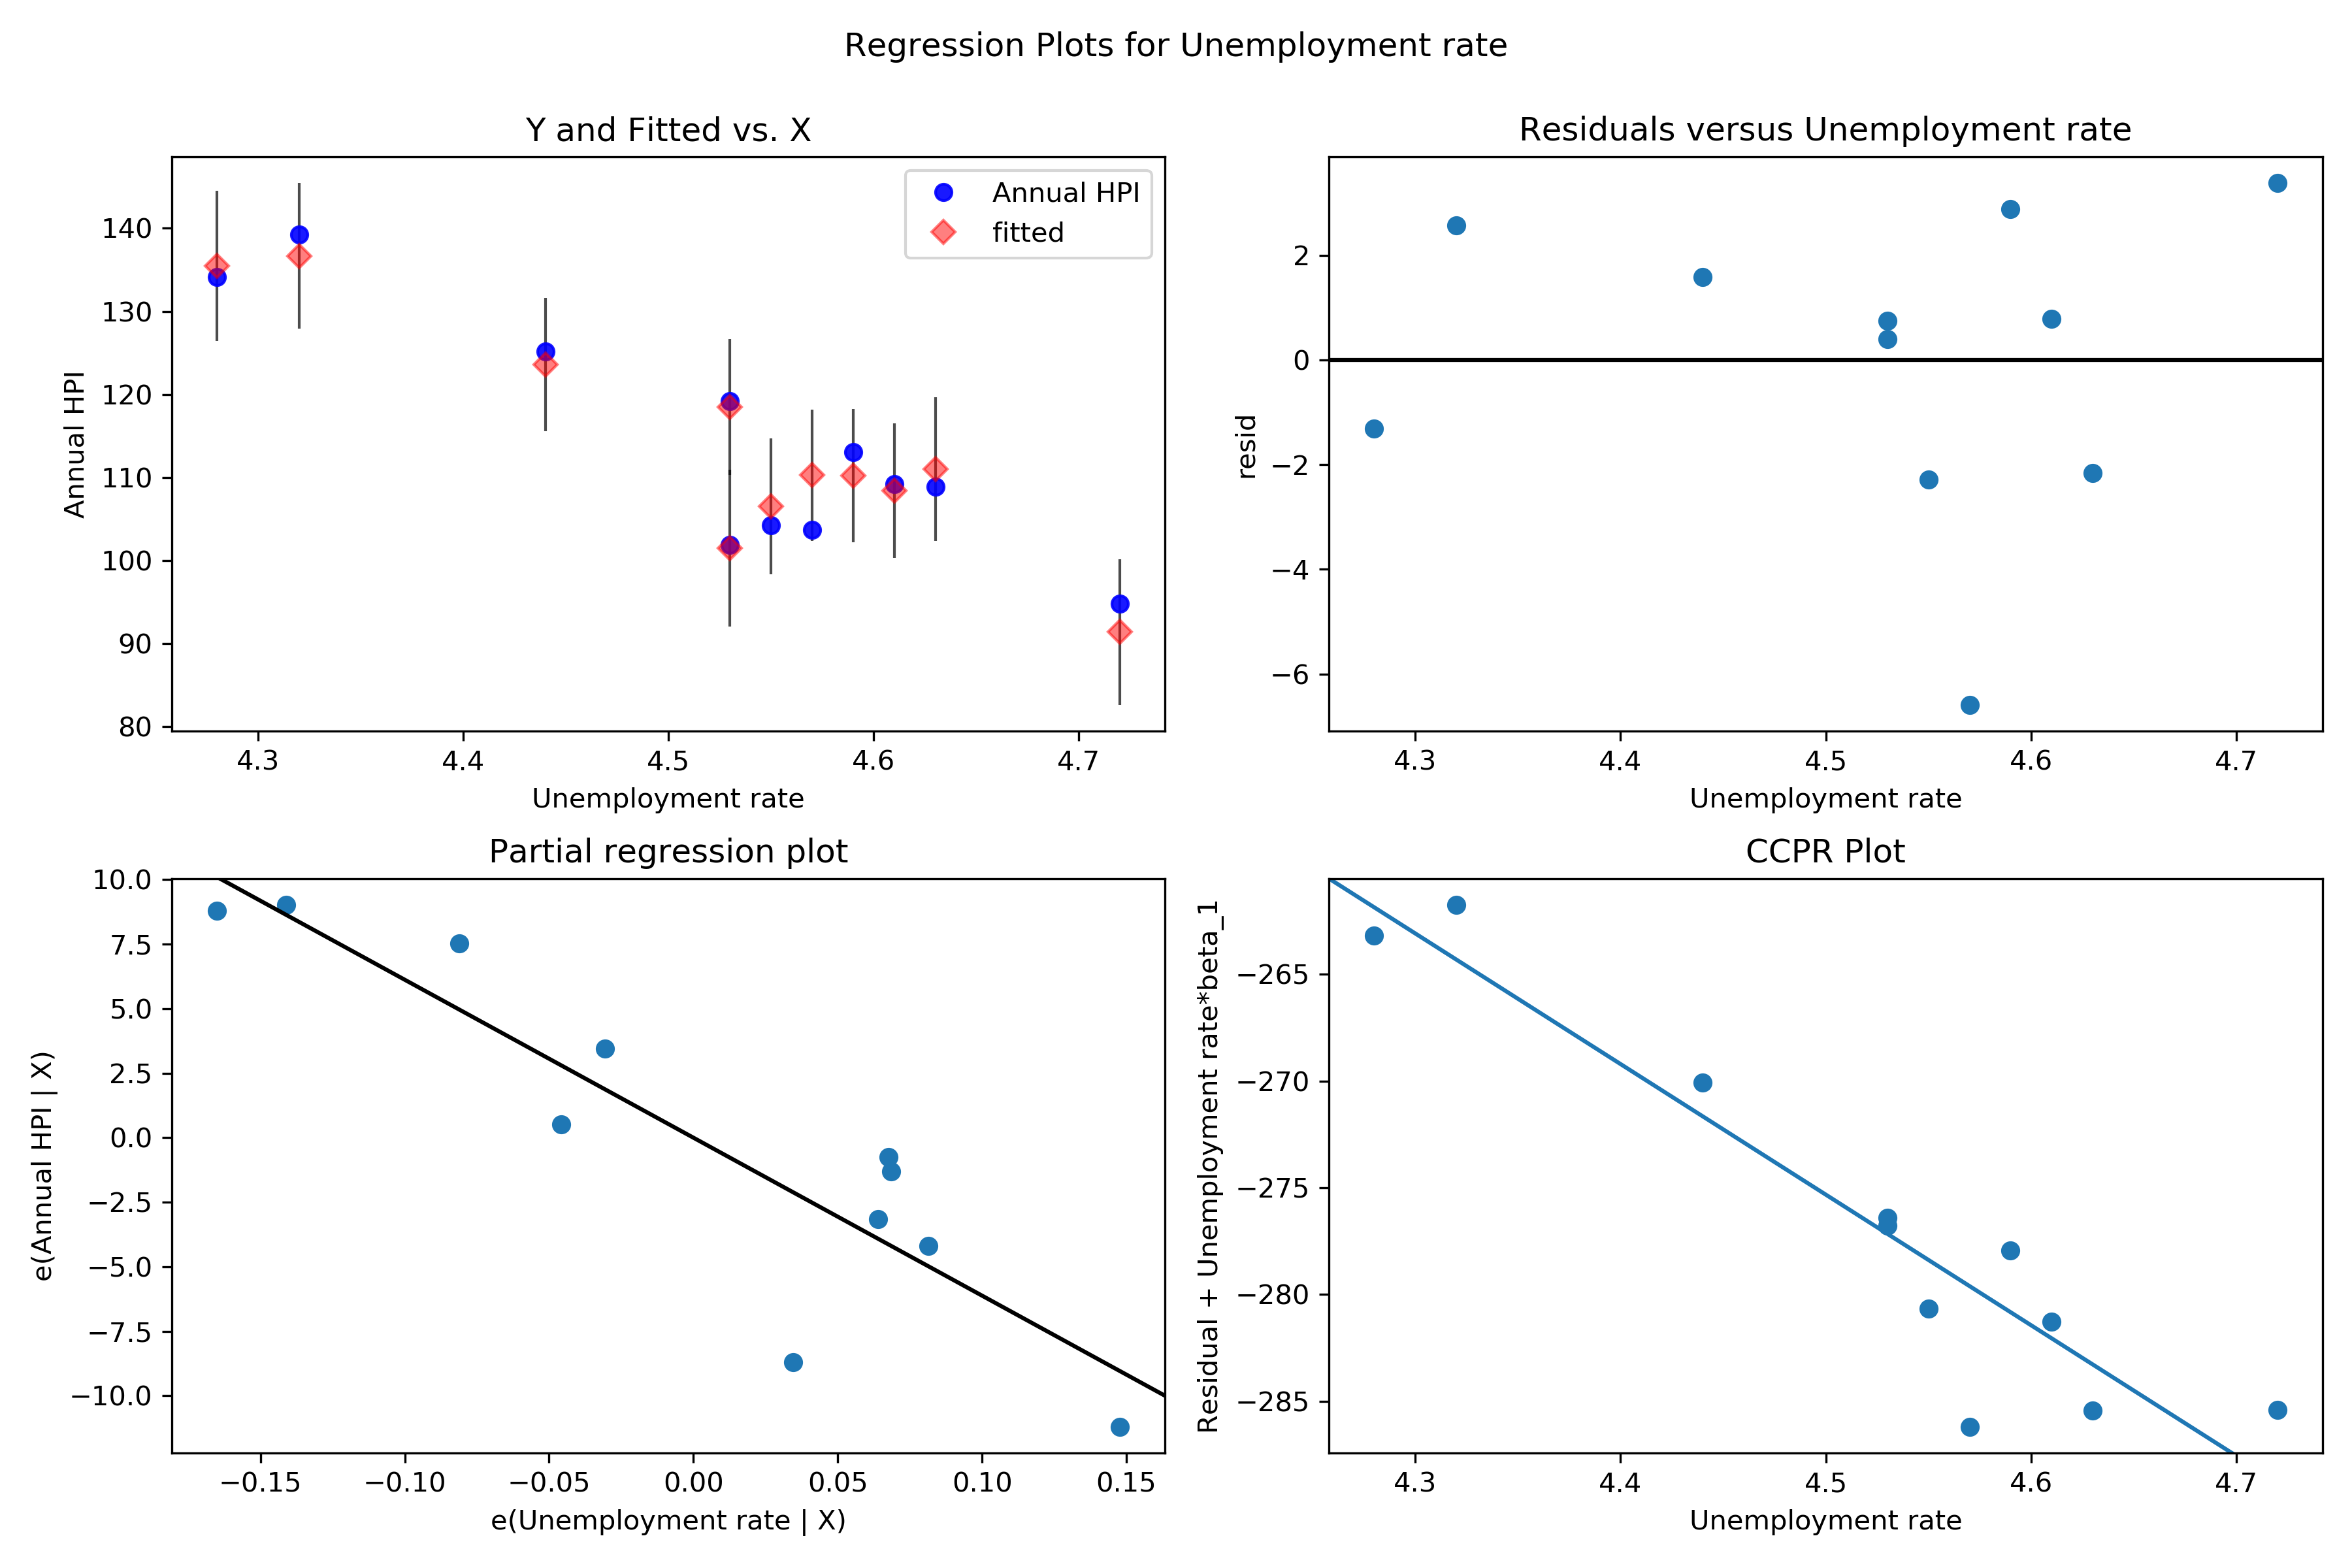
\includegraphics[width=0.49\textwidth]{./image/Resid_unemployment_CHN.png}}
\end{figure}

Philippines:
\begin{figure}[H]
\captionsetup[subfigure]{labelformat=empty}
\centering
\subfloat[]{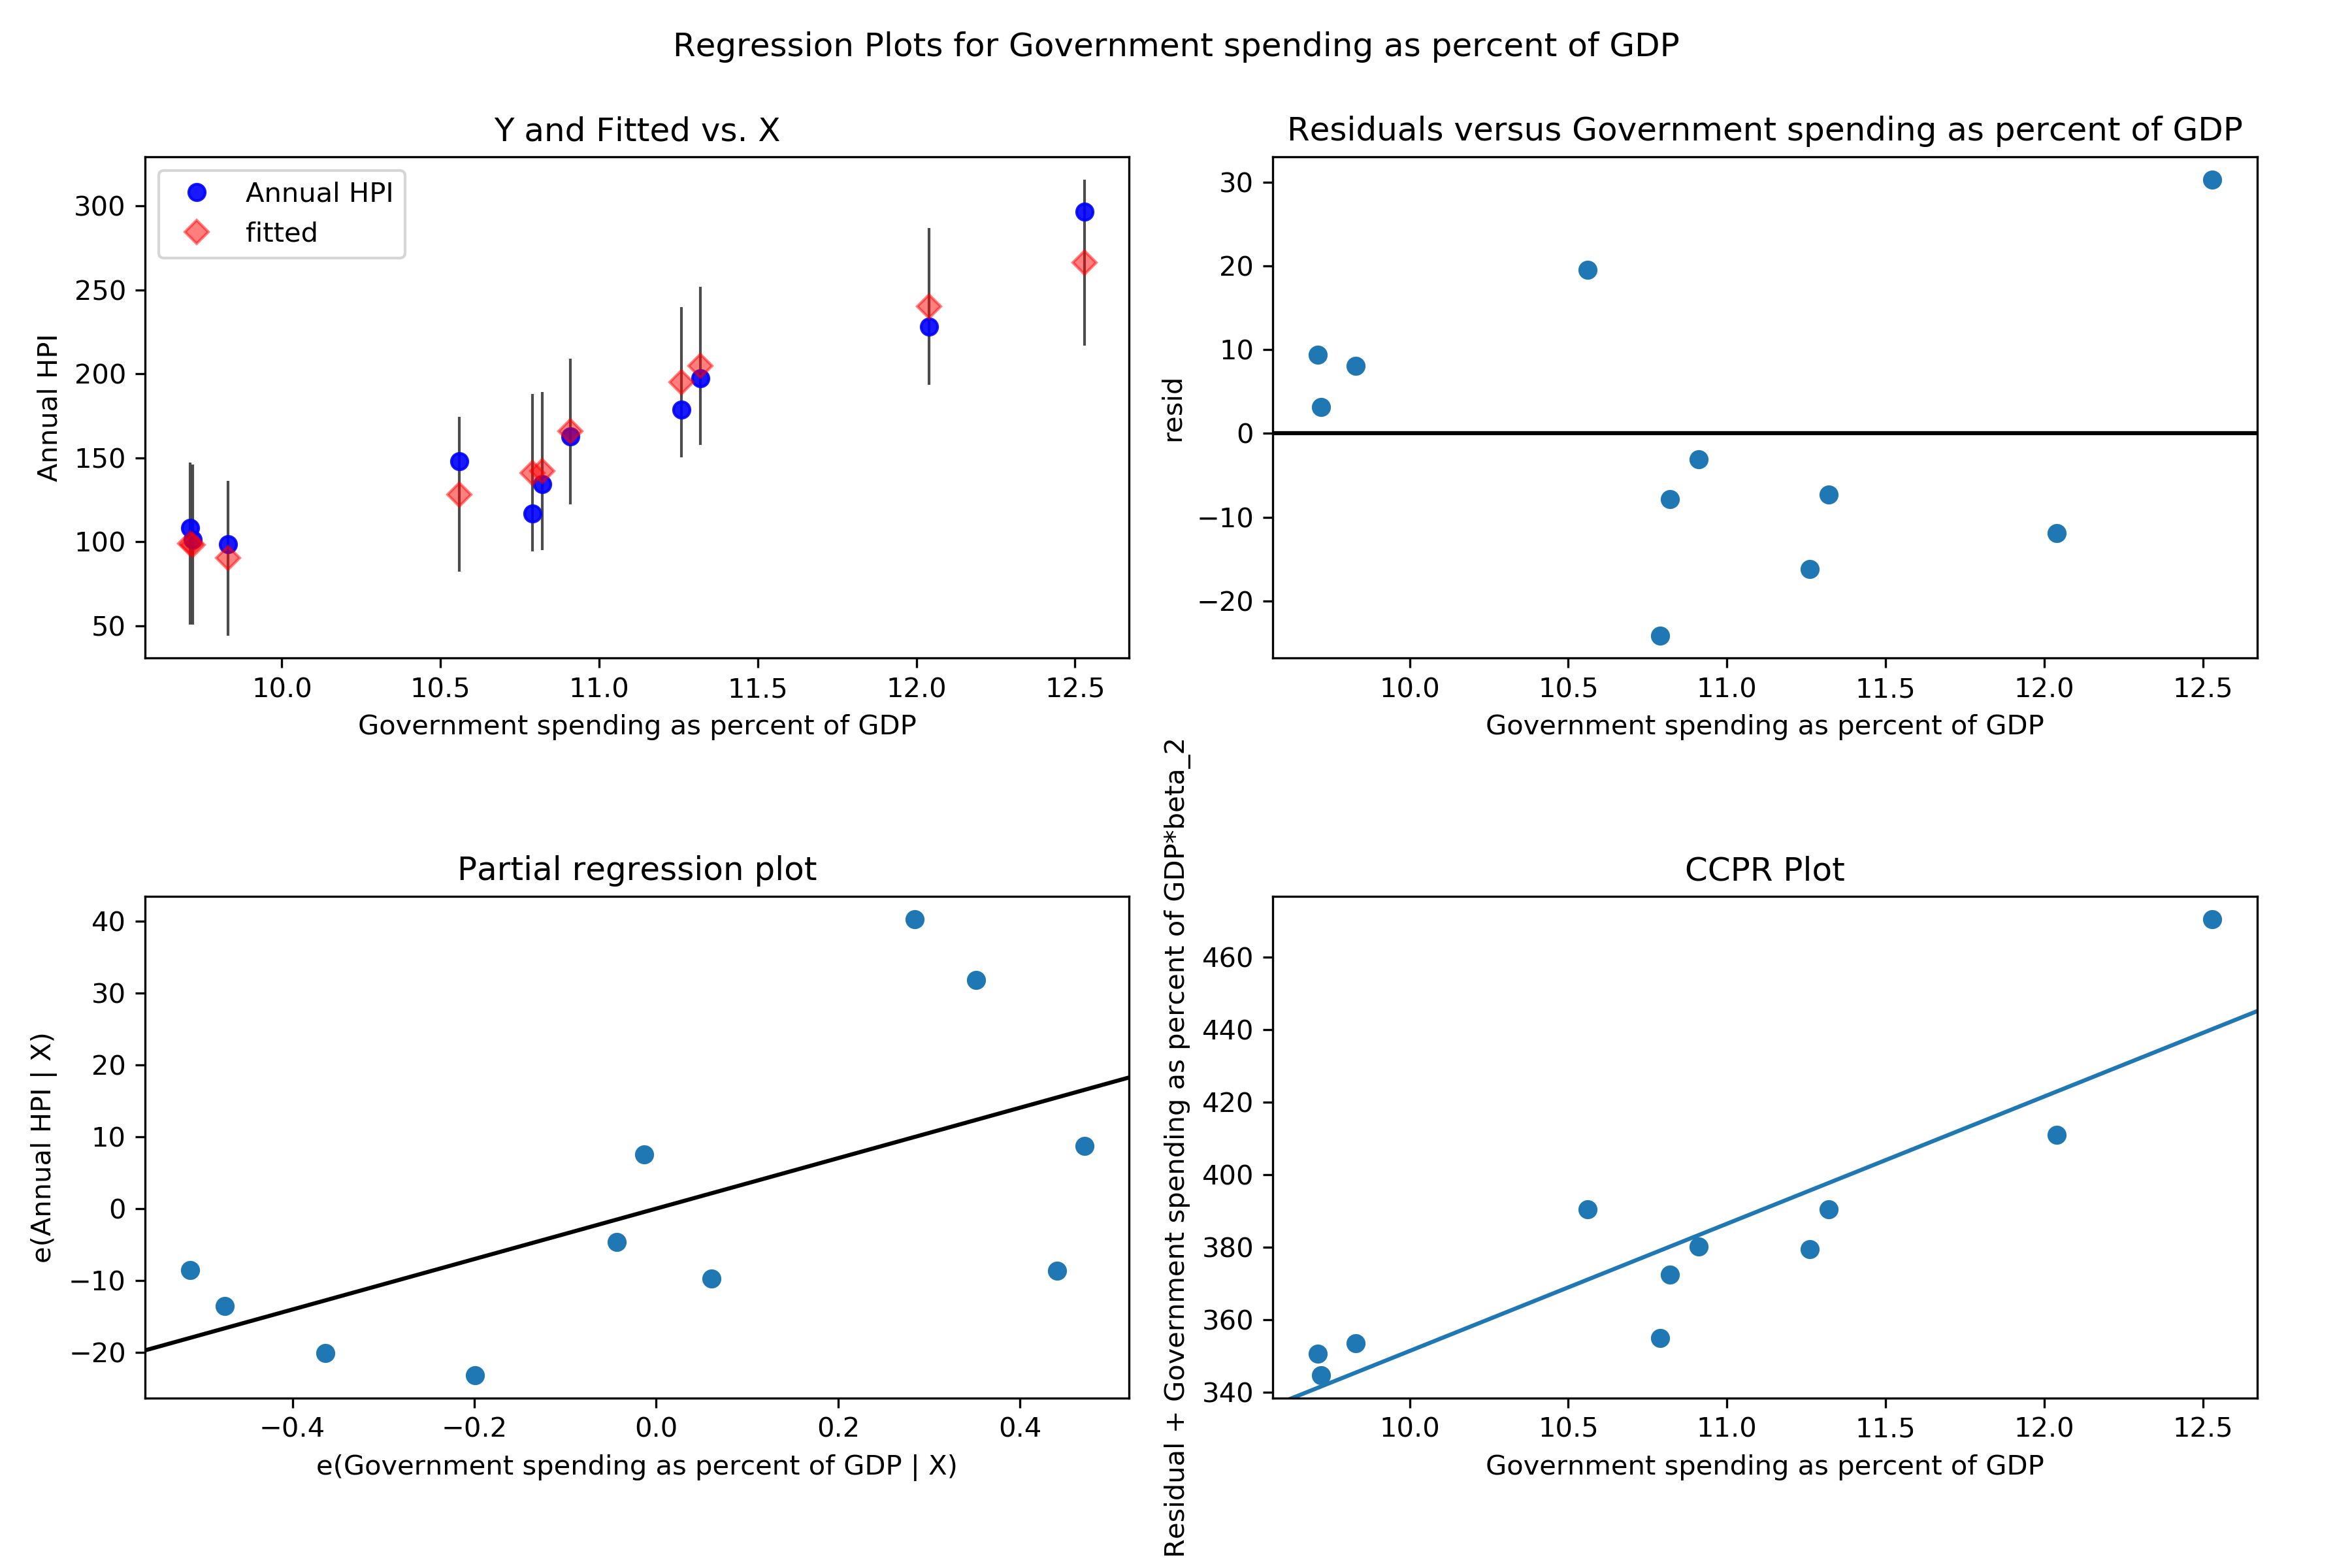
\includegraphics[width=0.49\textwidth]{./image/Resid_gs_PHL.png}}
\subfloat[] {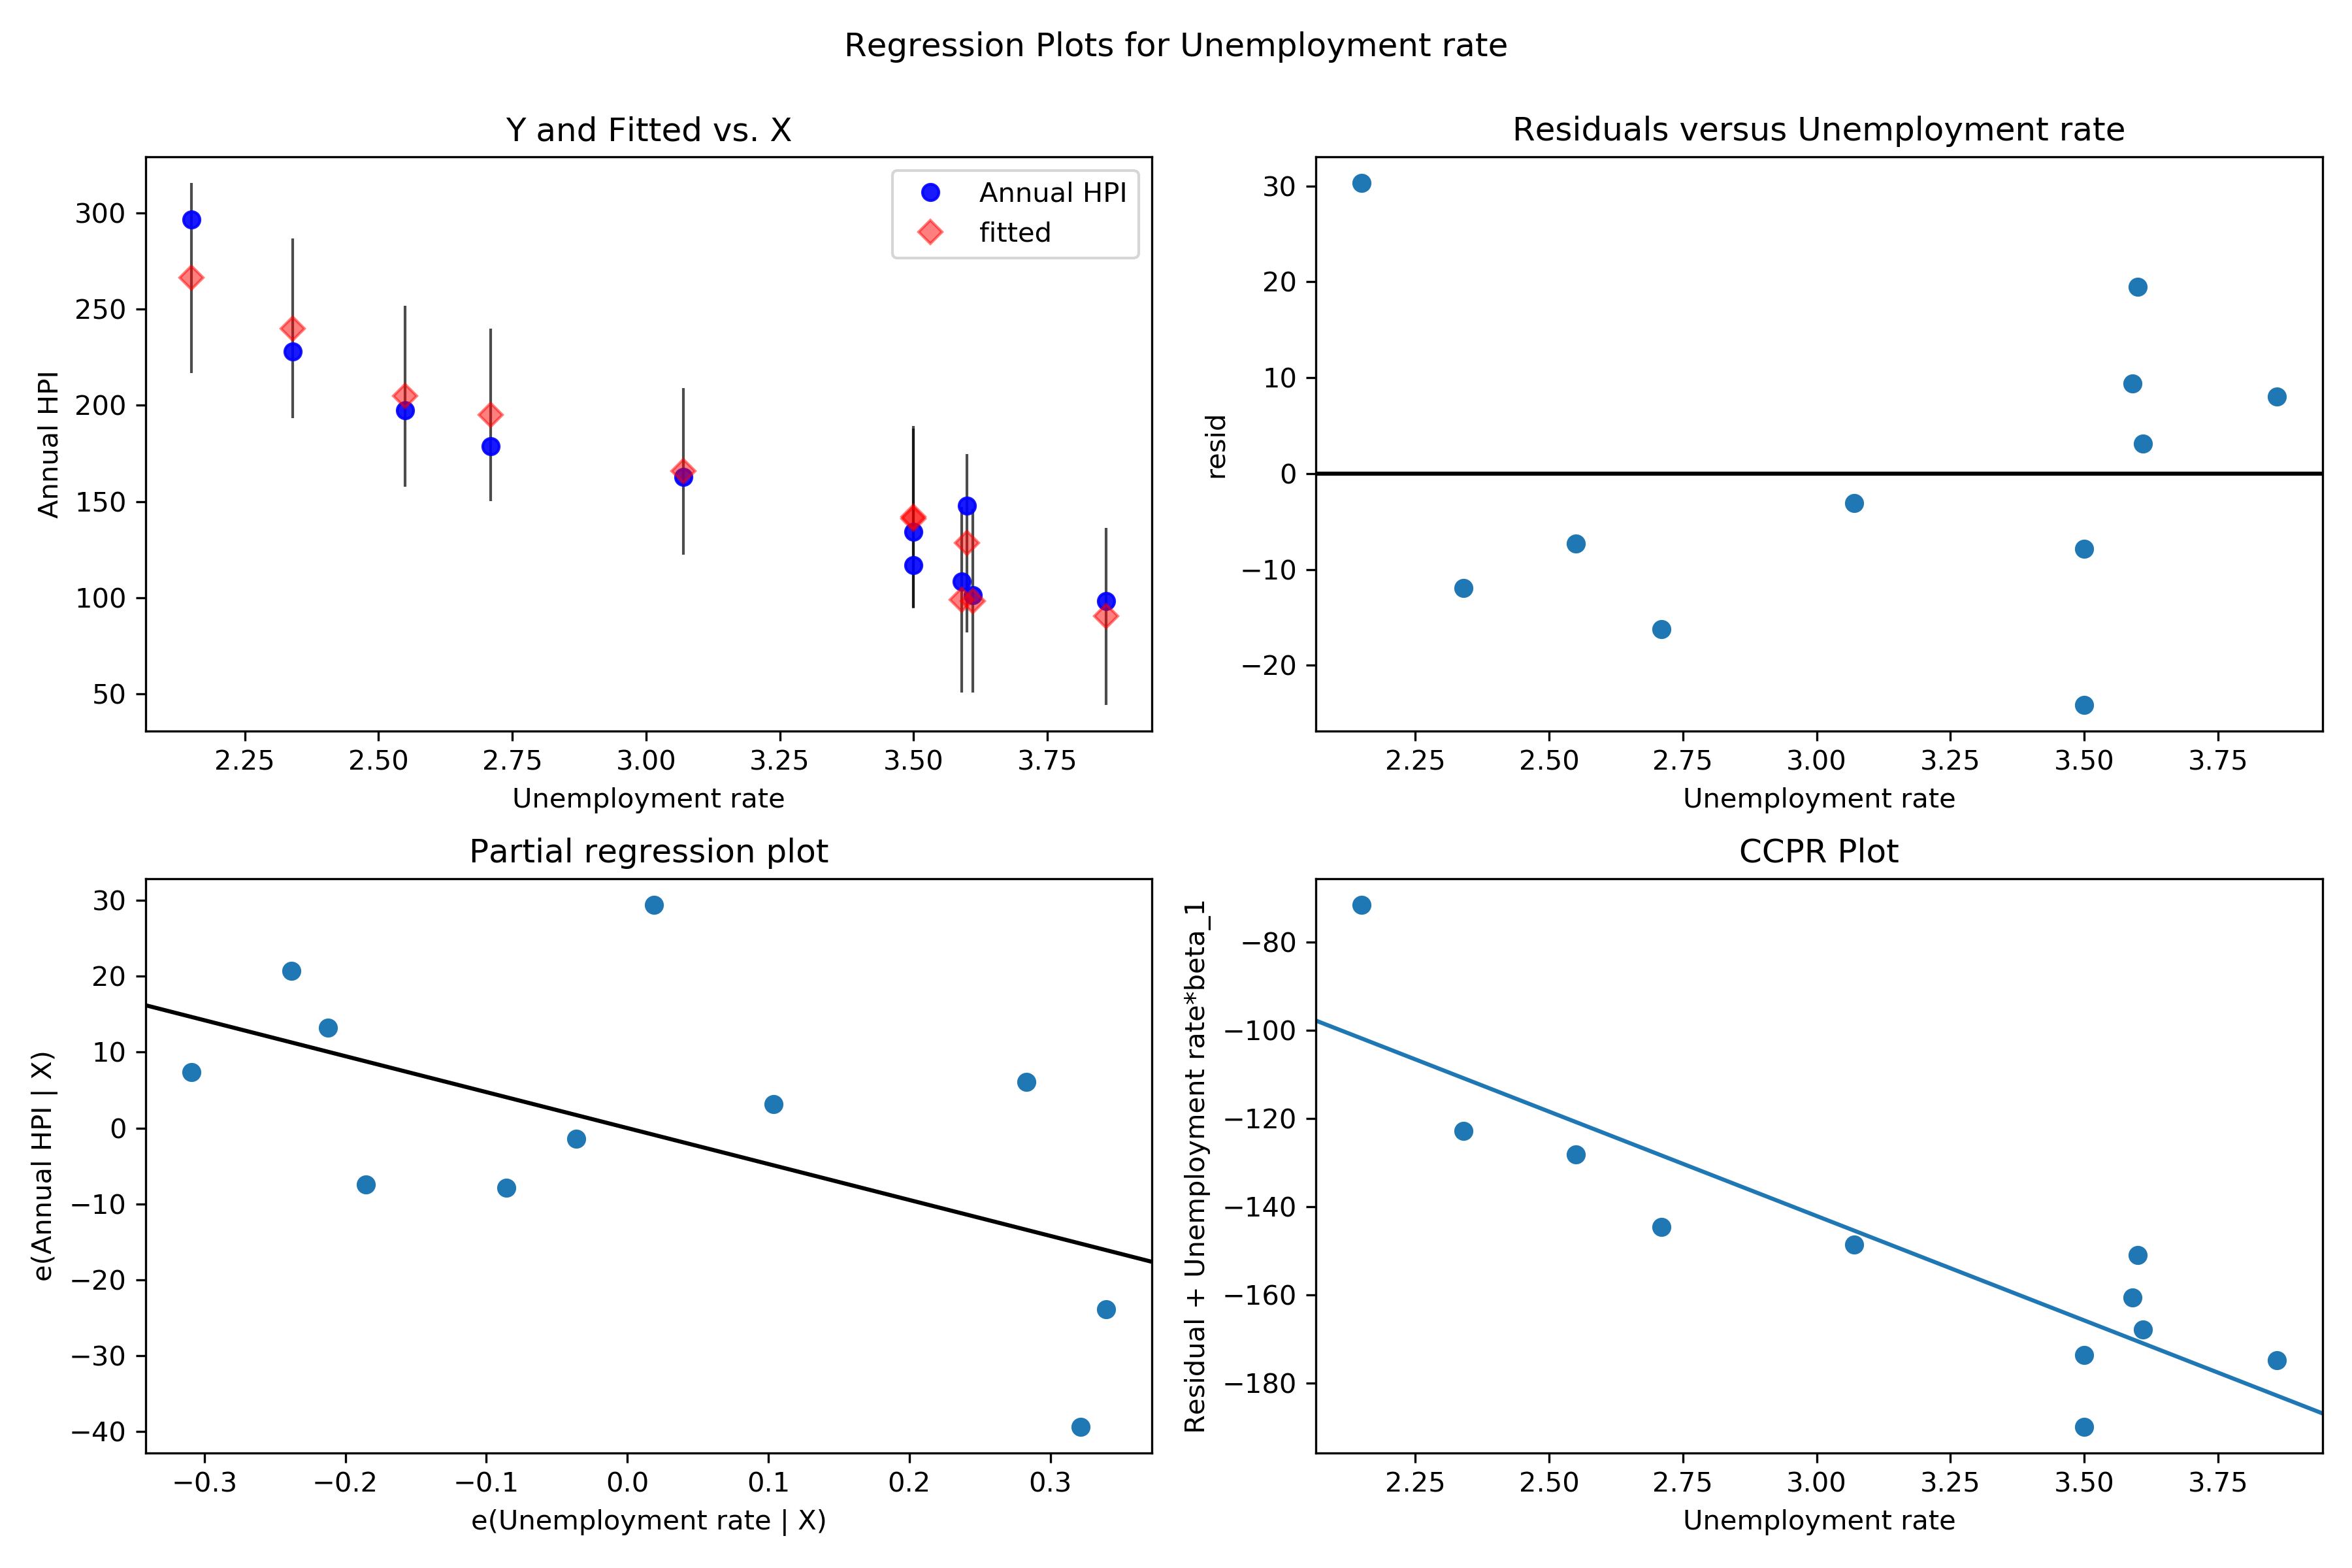
\includegraphics[width=0.49\textwidth]{./image/Resid_unemployment_PHL.png}}
\end{figure}

India:
\begin{figure}[H]
\captionsetup[subfigure]{labelformat=empty}
\centering
\subfloat[]{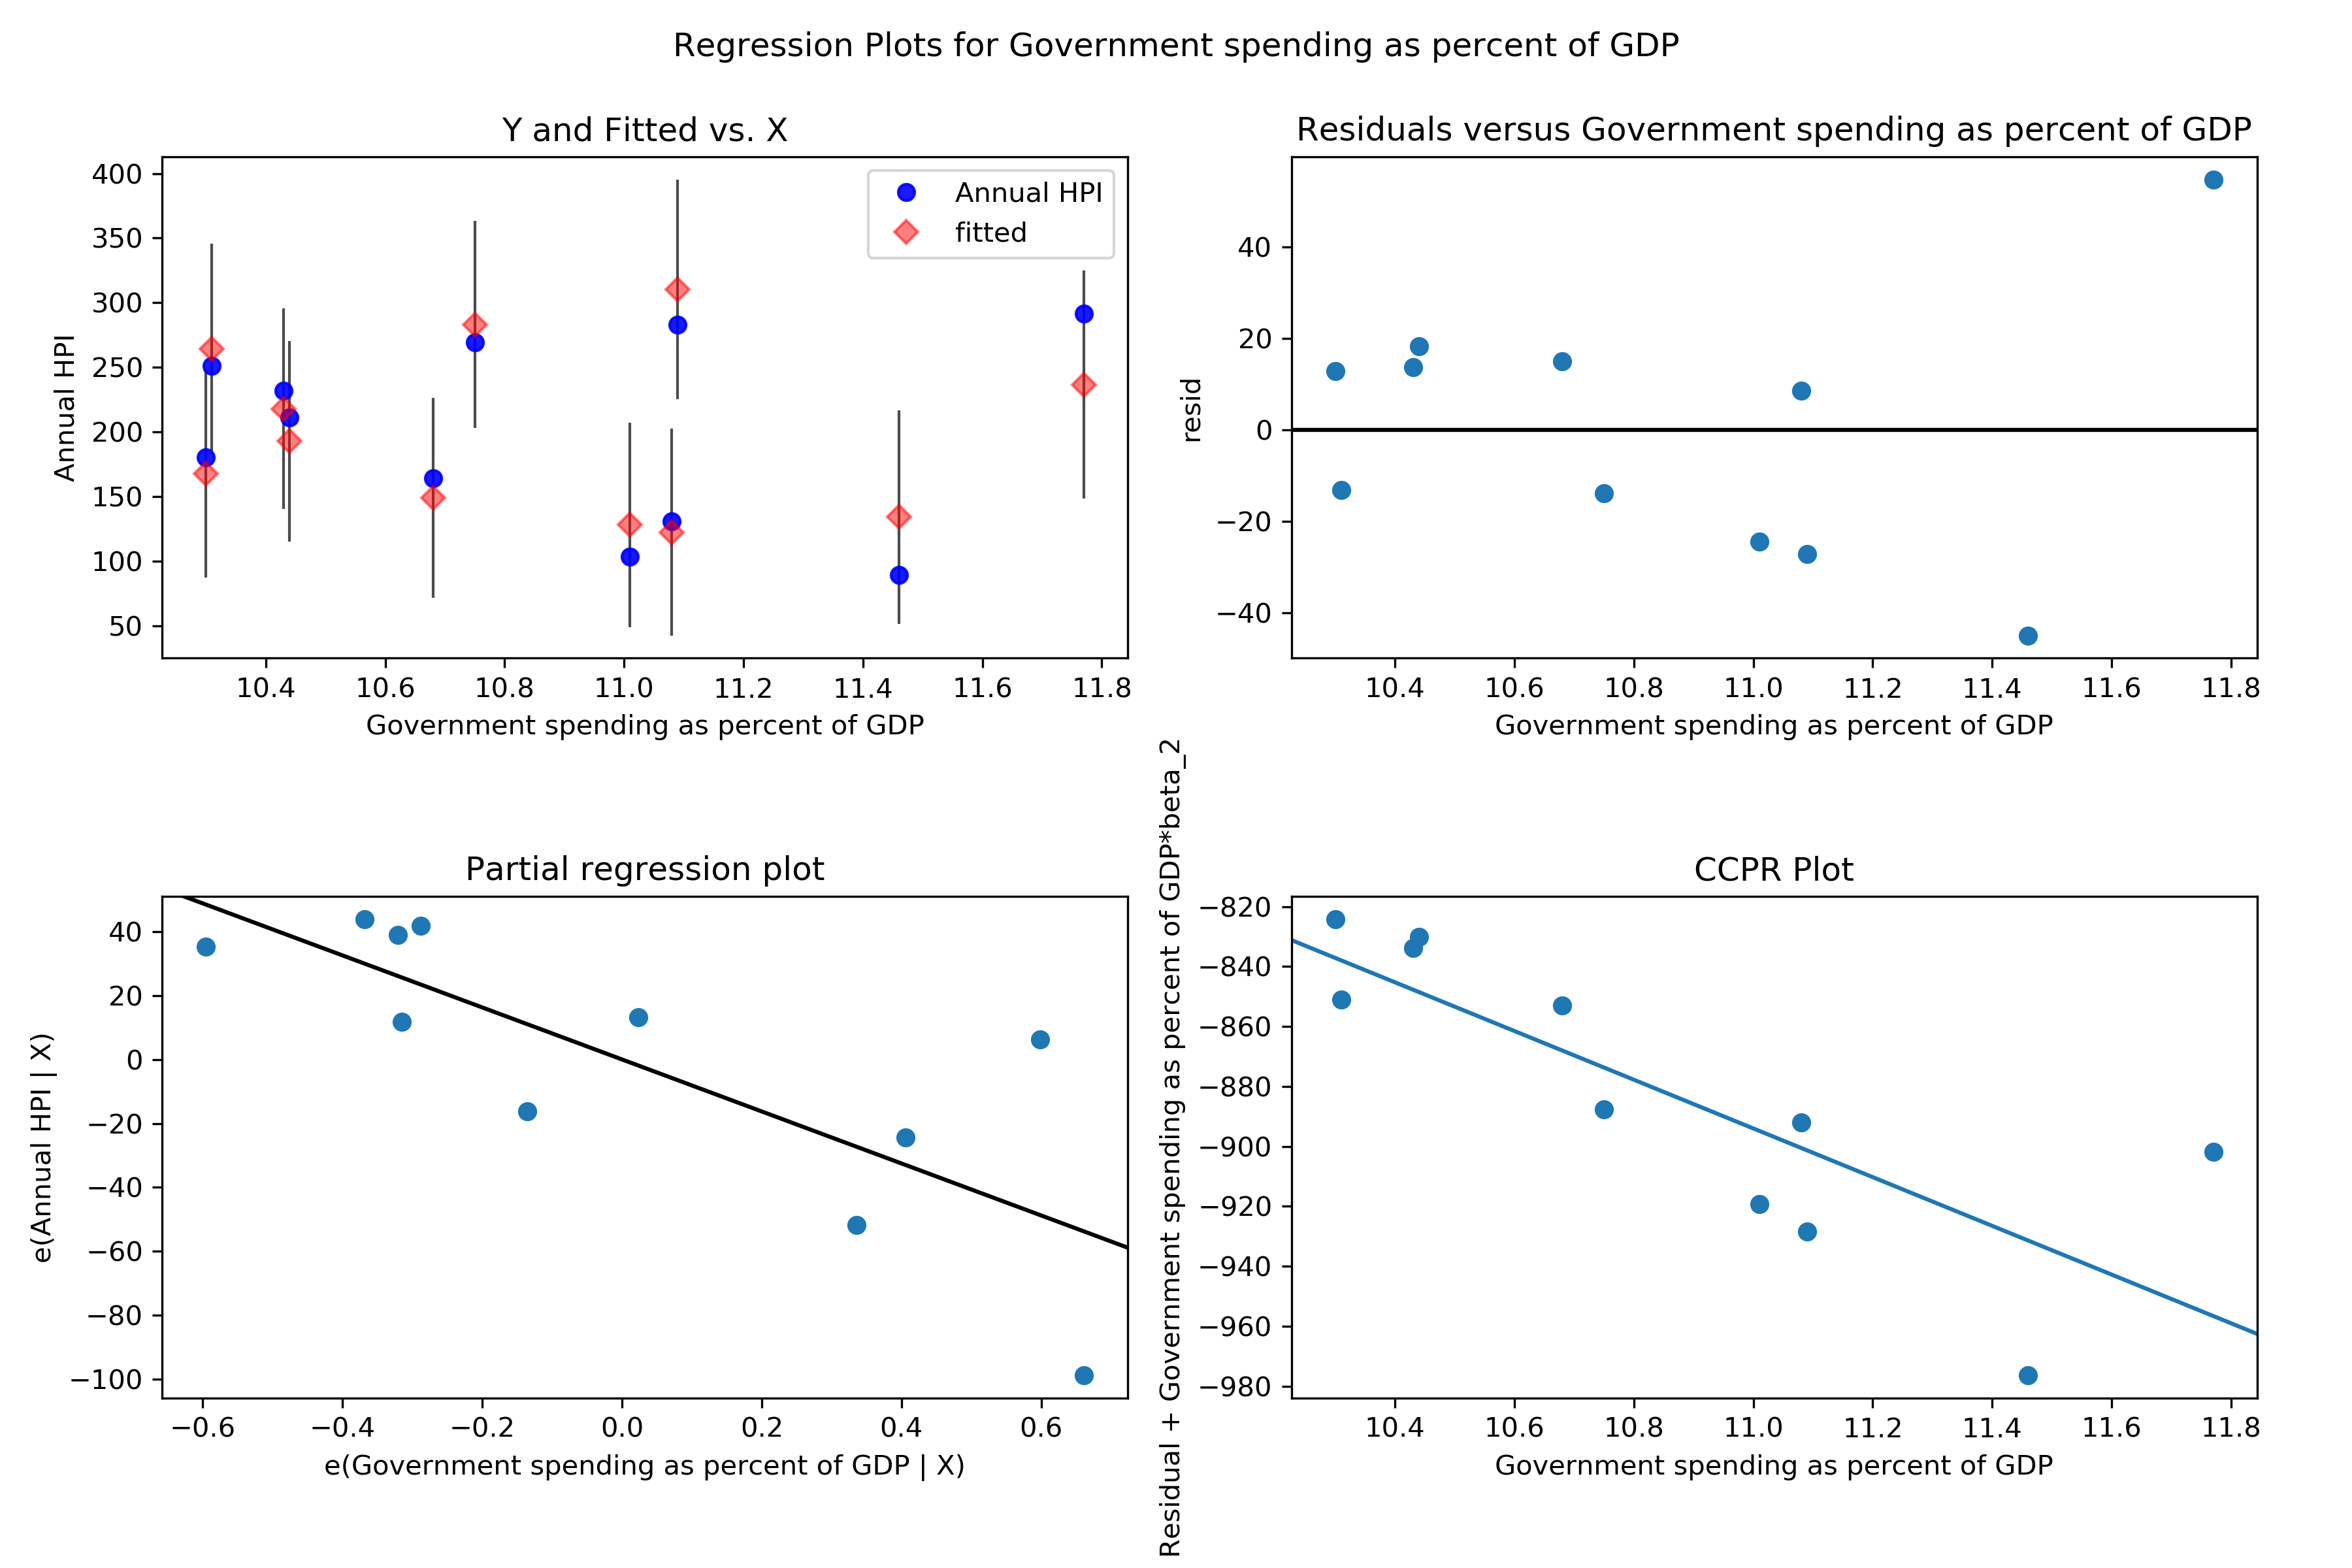
\includegraphics[width=0.49\textwidth]{./image/Resid_gs_IND.png}}
\subfloat[] {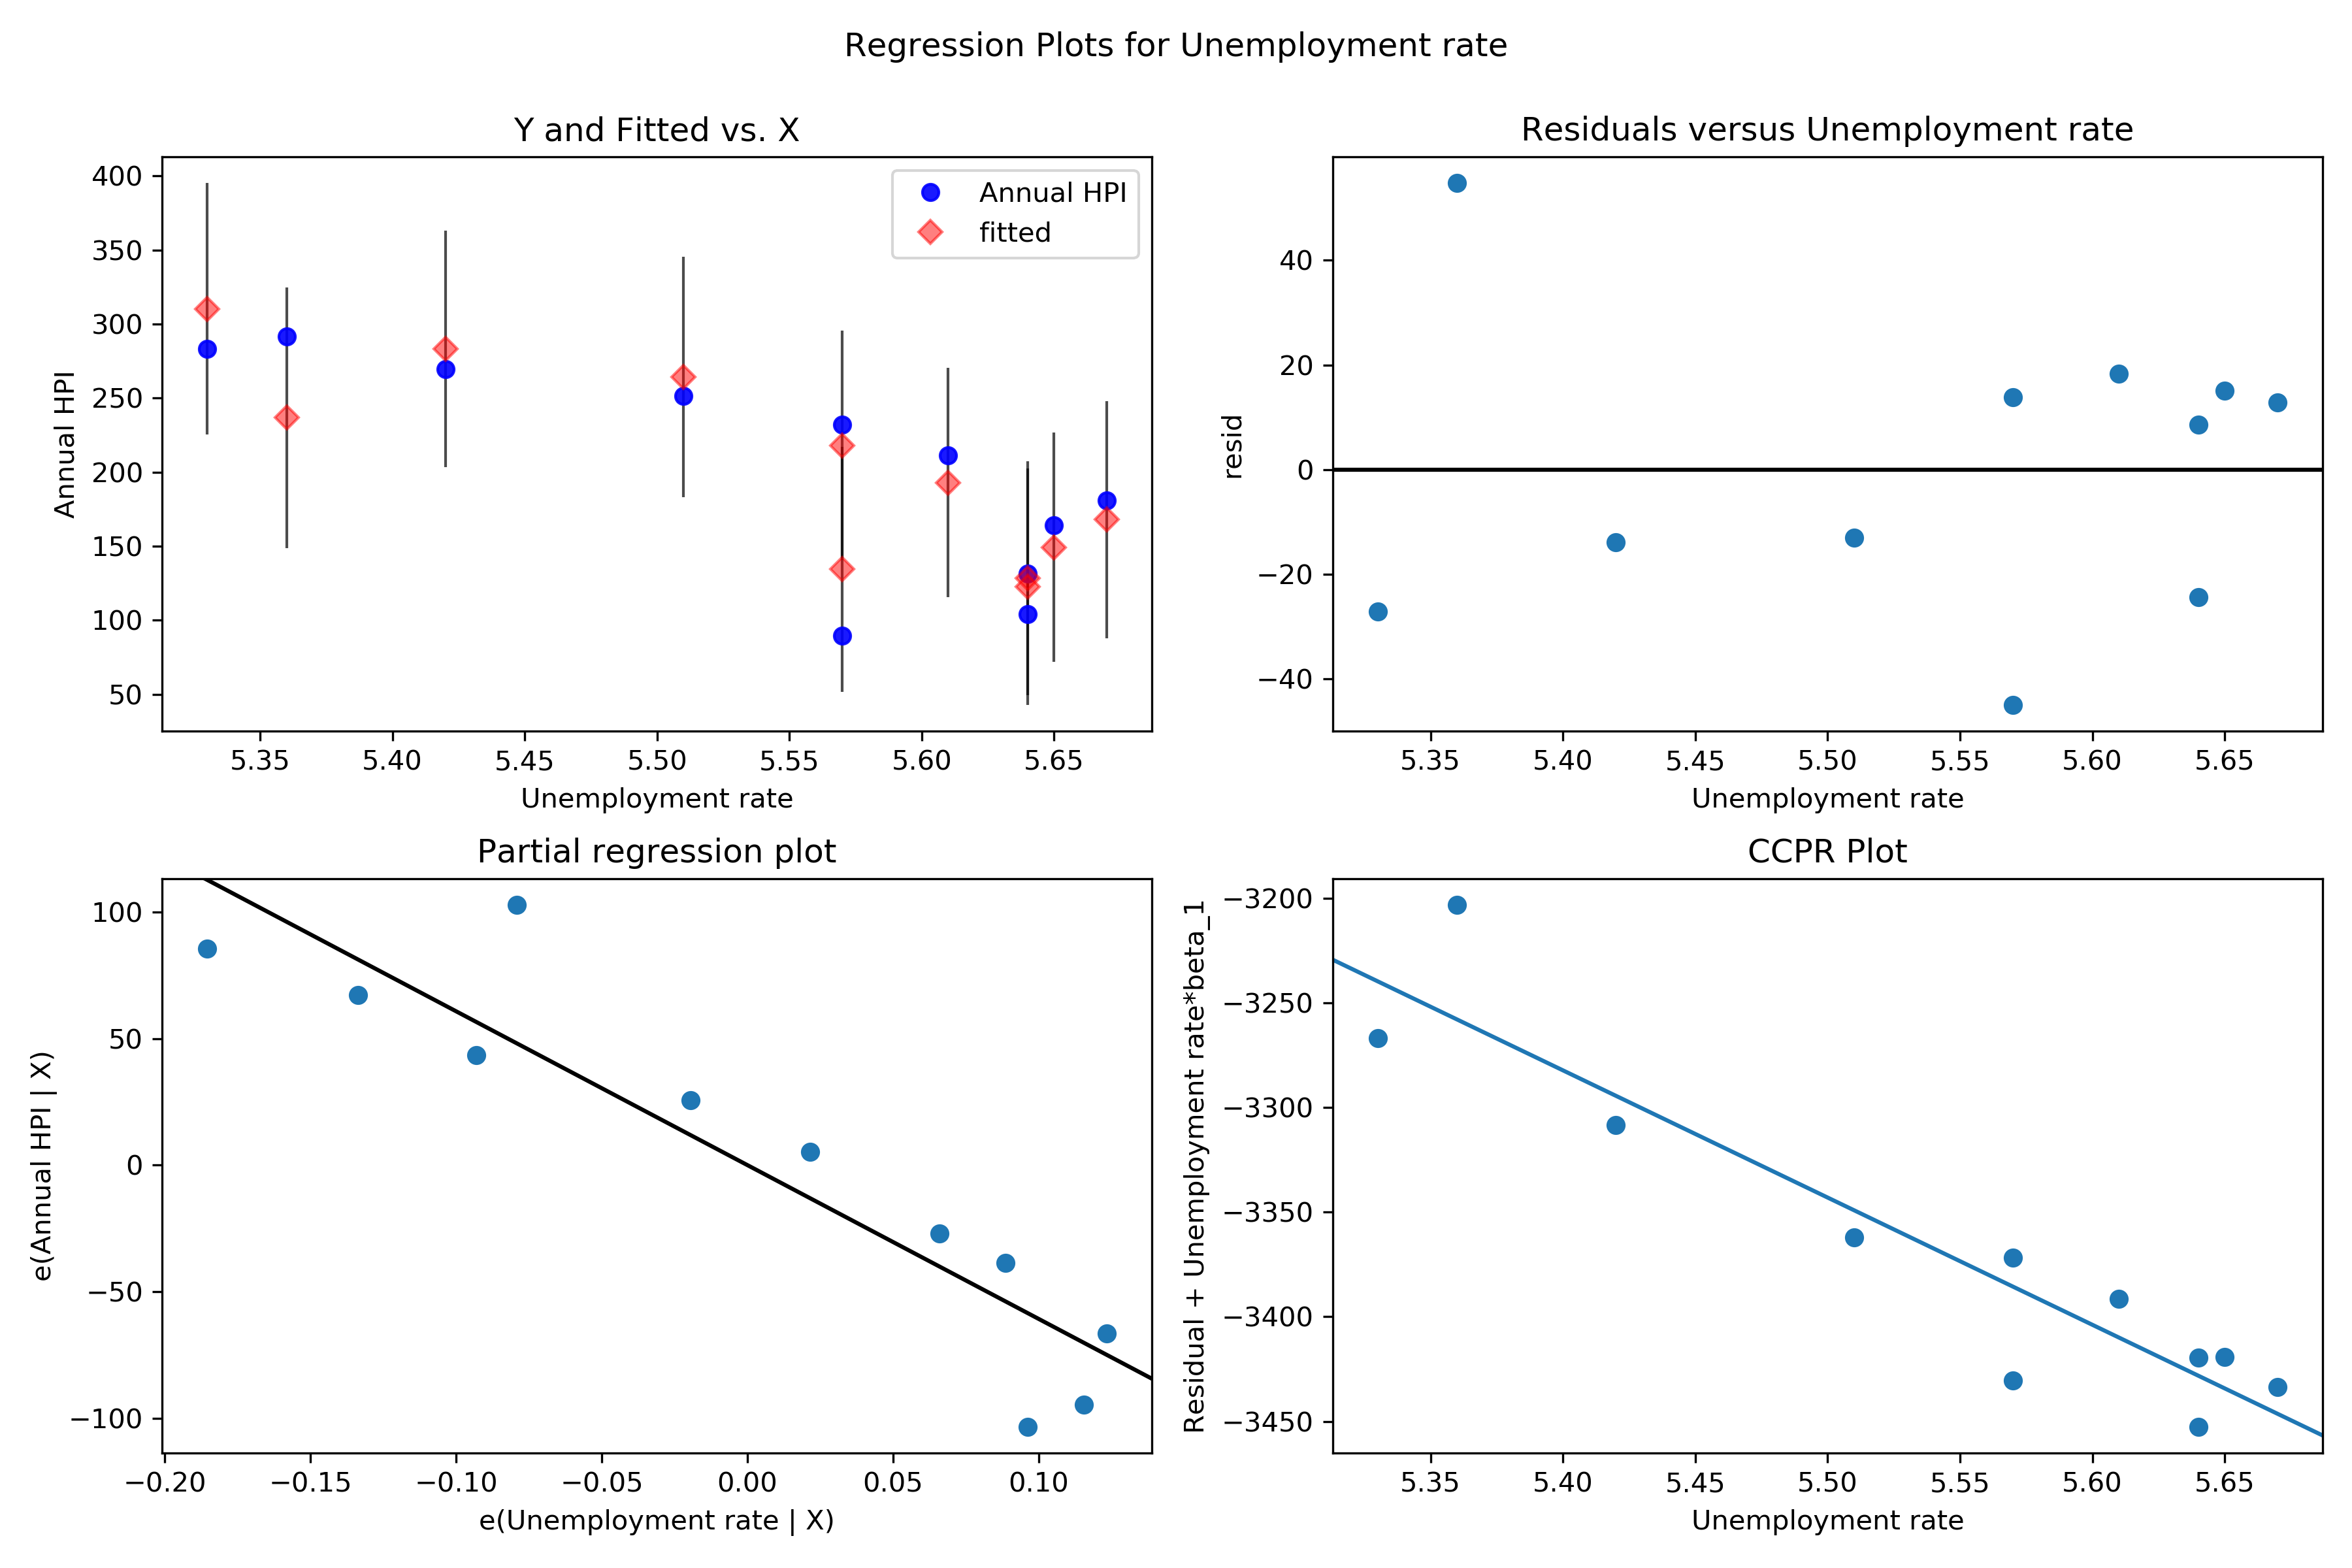
\includegraphics[width=0.49\textwidth]{./image/Resid_unemployment_IND.png}}
\end{figure}

For both unemployment rate and government spending as percent of GDP, the residuals for all four countries randomly scattered around zero (the upper right plots), which is an indication that heteroscedasticity is not a problem with either predictor variable in the model\citep{Residual1}.
\bibliographystyle{apalike}
\bibliography{references}

% https://stackoverflow.com/questions/39132469/how-to-interpret-scipy-stats-kstest-and-ks-2samp-to-evaluate-fit-of-data-t


\end{document}